\chapter{Introduction}
%--------------------------------------------------------
% Automata in general

Finite automata are a well-known model of computational theory used in many areas. Finite automata are commonly used in automata reasoning (e.g., in model checking \cite{DBLP:conf/cav/SiegelY20}, string solving and analysis \cite{DBLP:conf/popl/LinB16} or WS1S \cite{DBLP:conf/tacas/FiedorHJLV17, DBLP:journals/acta/FiedorHLV19}).

Finite automata are conceptually straightforward. However, operations on finite automata are often expensive: have high complexity, require extensive computational time and generate vast state space.

Our goal is to find different heuristics for optimizing several typical problems connected to finite automata. We study possibilities of using various abstractions of languages of finite automata states in optimization of automata algorithms. We abstract languages of states to sets of lengths of words in state languages and to Parikh images, represented as semi-linear sets, and explore options of using them to optimize the automata constructions by pruning states whose language abstractions represent an empty language. We work on optimizing performance of these abstractions. Moreover, besides optimization techniques specific for concrete state language abstractions, we also consider a general technique of mintermization to allow using our abstractions on additional structures such as regular expressions represented as finite automata and to optimize our abstractions further.

The idea of using abstraction in automata problem-solving is not new, but it is not properly explored either. There were first attempts of using abstraction techniques in automata such as alternating automata~\cite{GANTY20103444} or abstract regular model checking~\cite{method_model_checking_tool}, both using techniques similar to a general predicate abstraction~\cite{DBLP:conf/cav/ColonU98, DBLP:conf/cav/GrafS97} and CEGAR~\cite{DBLP:conf/cav/ClarkeGJLV00}.

We want to optimize operations on finite automata which take lots of computational time and generate vast state space. We are considering operations such as product construction, determinization of complement construction, minimization or determinization and inclusion test. Furthermore, we want to create state language abstractions which can work for different automata structures: operations on transducers, operations with alternating automata such as its emptiness or a conversion of an alternating automaton to its NFA representation, conversion of finite automata to flat automata, etc.

We focus on the construction of finite automata intersection generated by the synchronous product construction. We consider two common forms of this finite automata operation as our benchmark problems on which we test our optimizations:

\begin{itemize}
    \item first, construction of the intersection automaton by the synchronous product construction, which means completion of the entire product construction, and
    \item testing the emptiness of finite automata intersection (emptiness problem) which asks whether the language of the product is empty. Here, it is not always necessary to construct the entire product (or parts of the product) to resolve the emptiness of the intersection.
\end{itemize}

Nevertheless, even if our optimizations are introduced on product construction and emptiness problem, our discoveries have wider impact and are in some form applicable on many typical automata operations.

%--------------------------------------------------------
% Intersection

The intersection of finite automata combines the original states from the individual automata to tuples called product states in the generated state space by finding corresponding transitions with the same symbols. Every product state represents an intersection of languages of the corresponding states in the original automata. The synchronous product construction is computationally costly: for two finite automata, the generated product state space can increase quadratically to the number of input finite automata states (number of states in one finite automaton times number of states in the second finite automaton) and transitions. And, for multiple finite automata, exponentially to the number of used finite automata. However, there are often large parts of the generated state space which cannot accept any words (no final states can be reached from these states), yet are still generated\footnote{The generated product state space sometimes \emph{explodes}.}. Therefore, it is important to have a decent algorithm to minimize the generated product state space as much as possible.

%--------------------------------------------------------
% Our optimization

In our optimizations, we try to identify which generated product states cannot lead to any accepting state or are successive only to such states. When state language abstractions of states in product state are not compatible---the original languages of the corresponding states cannot accept the same words---we can omit such product state and all their potential successive states, pruning the generated state space.

%--------------------------------------------------------
% Length abstraction

We start with an optimization using length abstraction of state languages. For each state, we construct a so-called lasso automata. It is used to compute a semi-linear formula which codes the lengths of the words in the languages of current states (we call them accepted lengths). We use SMT solver to resolve satisfiability of these formulae. When accepted lengths of states in the product states are not compatible (their formulae are not satisfiable), their languages have no common words. There is no path from the product state leading to the accepting product state. We can prune such product states. Consequently, this removes the need to even consider their potential successive states.

Even though there still might be states which do not lead to any final state in the final product, this simple optimization often trims substantial parts of the state space. Length abstraction can also be implemented simply and efficiently. However, sometimes the abstraction is too coarse. For instance, it cannot detect unnecessary product states for finite automata with rich alphabets, since their states accept a multitude of word lengths.

%--------------------------------------------------------
% Parikh image

For that reason, we investigate a finer state language abstraction which uses Parikh images of state languages. Parikh image of a word tells us how many times each symbol occurs in the word\footnote{A function which assigns each transition symbol a number of occurrences in a word.}. Parikh image of a language is a semi-linear formula describing the relation between the number of symbol occurrences in words in a language. In contrast to the length abstraction, it contains additional information about the numbers of symbols in words. We can more precisely identify unnecessary state space by determining compatibility of Parikh image abstractions. To solve satisfiability of their formulae, we use SMT solver. However, the Parikh image computation is expensive. There is a trade-off between the precision of the Parikh image abstraction and its cost.

Generating smaller state space using our Parikh image optimization can improve computation time for the product generation in case substantial parts of the state space are pruned. Moreover, it is even enough to decide the emptiness of the intersection on the initial product state immediately in many cases.

%--------------------------------------------------------
% Specific optimizations for state language abstractions.

An important part of this work is researching optimizations of the specific state language abstractions to make their usage efficient. For both abstractions, we find a way to skip evaluation of state language abstractions for product states in long \emph{lines} (linear non-branching sequences of states). If a product state with compatible accepted lengths generates a single sequence of states, all states in the line have compatible length abstractions.

For length abstraction, we reduce lasso automata generation for each state to a single expanding lasso automaton for the whole finite automaton. We also efficiently evaluate length abstractions without SMT solver by resolving satisfiability of their formulae with a special construction using linear congruences.

For Parikh image computation, we remove parts of Parikh image formula, which can reduce its precision, but it occurs that it has no impact on pruning capabilities on our benchmark automata. The formulae are large. However, extensive parts of them remain unchanged for different product states. We utilize incremental SMT solving to precompute the common parts and for each state recompute only the remainder of the formulae. This speeds up the evaluation of compatibility of Parikh image abstractions. If resolving satisfiability of formulae takes too long, we can introduce a timeout for SMT solver to stop the computation and not prune the product state.

We also consider combinations of our abstractions, particularly we experiment with computing cheap length abstraction first and computing the Parikh images only when length abstraction fails to prune product states.

%--------------------------------------------------------
% Mintermization

Further, we use mintermization for intersection of finite automata as a different approach to processing the initial automata before applying other optimizations. We compute minterms, which can be used instead of transition symbols while retaining all information about the automata to compute Parikh images and other optimization abstractions faster.

%--------------------------------------------------------
% Experiments + Contributions

We implement the proposed abstractions and evaluate their impact on the emptiness problem and the product construction experimentally. We experiment with a benchmark containing a set of different finite automata obtained from runs of a regular model checking tool on verification of pointer programs and parametric protocols created in~\cite{model_checking_tool_10.1007/978-3-540-70844-5_7} based on a method of abstract regular model checking from~\cite{method_model_checking_tool}. We generate products of various combinations of these finite automata and solve the emptiness problem of their intersections or generate the whole products. We focus on the number of trimmed product states and their nature, their position in the product or other significant properties. For certain types of automata, our optimizations work really well. Parikh image abstraction usually trims vast state spaces where length abstraction cannot prune everything and unoptimized product state space explodes (e.g., from $20000$ to $10$ product states). In addition, the abstractions are sometimes successful at immediately stopping product construction on the first initial product state if the intersection is empty, while, in some cases, product construction would take hours (in one case, more than 7 hours, compared to 1 minute with Parikh image abstraction).

The contribution of this work can be summarized as follows:
\begin{enumerate}
    \item heuristics trimming the generated state space of finite automata operations based on abstractions of specific state languages: length abstraction and Parikh image computation; or general approaches as mintermization,

    \item optimizations for explored state language abstractions:
    \begin{itemize}
        \item skipping evaluation of state language abstractions for some product states for sequences of product states in long lines,
    \end{itemize}

    \item optimizations specific for length abstraction:
    \begin{itemize}
        \item generating a single lasso automaton for the whole finite automaton,
        \item efficient evaluation of length abstraction without SMT solver,
    \end{itemize}

    \item optimizations specific for Parikh image abstraction:
    \begin{itemize}
        \item reduced Parikh image to resolve satisfiability of Parikh image formulae faster,
        \item resolving Parikh images with incremental SMT solving,
        \item resolving Parikh images with a timeout for SMT solver,
    \end{itemize}

    \item combination of state language abstractions to optimize automata problems, and

    \item implementation and experimental evaluation of said heuristics and their optimizations.
\end{enumerate}

%--------------------------------------------------------
%--------------------------------------------------------
%--------------------------------------------------------
%--------------------------------------------------------

\chapter{Preliminaries}

Let us clarify a few definitions and terms often used throughout this paper. The following definitions are mostly adapted from~\cite{Esparza} or~\cite{Sipser}.

\emph{Alphabet} is a finite, non-empty set denoted by $\Sigma$. Elements of an alphabet are called \emph{symbols} or \emph{letters}. A finite, possibly empty, sequence of symbols over an alphabet is a \emph{word} $w$ from the set of all words $\Sigma^*$ over an alphabet $\Sigma$.

\begin{definition}[\textbf{Deterministic finite automaton}] \hfill \newline
    A deterministic finite automaton (DFA) is a 5-tuple $A = (Q, \Sigma, \delta, I, F)$, where:
    \begin{itemize}
        \item Q is a non-empty \textbf{set of states},
        \item $\Sigma$ is an \textbf{input alphabet},
        \item $\delta$ is a \textbf{transition function}: $Q \times \Sigma \rightarrow{} Q$,
        \item $I \in Q$ is an \textbf{initial state}, and
        \item $F \subseteq Q$ is a \textbf{set of final (accepting) states}.
    \end{itemize}
\end{definition}

A \emph{run} of $A$ on input $a_0a_1a_2 \ldots a_{n-1}$ is a sequence $q_0 \xrightarrow{a_0} q_1 \xrightarrow{a_1} q_2 \xrightarrow{a_3} \ldots \xrightarrow{a_{n-1}} q_n$, such that $q_i \in Q$ for $0 \leq i \leq n$, $q_0 = I$ and $\delta(q_i, a_i) = q_{i+1}$ for $0 \leq i \leq n - 1$. A run is \emph{accepting} if $q_n \in F$. $A$ \emph{accepts} a word $w \in \Sigma^*$ if $A$ has an accepting run on input $w$. A \emph{language} recognized by $A$ is a set $L(A) = \{w \in \Sigma^* \,\vert\, w \text{ is accepted by } A\}$. A single \emph{transition} from $\delta$ is denoted as $q \xrightarrow{a} q'$ if $q' \in \delta(q, a)$ and means \textit{one can get from state $q$ to state $q'$ with a transition symbol $a$}. For every state, DFA has at most one transition for a given symbol. Consequently, DFA has exactly one run on a given word from initial state to one of the accepting states (or non-terminating states\footnote{No accepting state is accessible from them.} in case the word is not accepted by the automaton at all).

\begin{definition}[\textbf{Non-deterministic finite automaton}] \hfill \newline
    A non-deterministic finite automaton (NFA) is a 5-tuple $A = (Q, \Sigma, \delta, I, F)$, where $Q$, $\Sigma$ and $F$ are as for DFA and:
    \begin{itemize}
        \item $\delta$ is a \textbf{transition relation}: $\delta: Q \times \Sigma \rightarrow{} P(Q)$, where $P(Q) = \{R \,\vert\, R \subseteq Q\}$ is a set of subsets of $Q$, and
        \item $I = \{q \,\vert\, q \in Q\}$ is a non-empty \textbf{set of initial states}.
    \end{itemize}
\end{definition}

For every state and its transition symbol, $P(Q) \in \delta(q, a)$ is a singleton. For example, $\delta(q_1, a) = \{ q_1, q_2 \}$.

Two finite automata $A_1$ and $A_2$ are said to be \emph{equivalent} when both accept the same language: $L(A_1) = L(A_2)$.

For every NFA $A$ exists a corresponding equivalent DFA $A'$. \emph{Determinization} is a process of converting such NFA to DFA.

\begin{definition}[\textbf{Powerset (\textbf{subset}) construction}] \hfill \newline
    The powerset construction is a method for creating a corresponding deterministic finite automaton from its equivalent non-deterministic finite automaton. Produces finite automaton $A'$, where $Q' = 2^Q$, $F' = \{S \in Q' | S \cap F \neq \emptyset\}$, $I' = I$ and for $S \in Q': \delta'(S, a) = \bigcup_{s \in S} \delta(s, a)$.
\end{definition}

\begin{definition}[\textbf{Product construction}] \hfill \newline
Given two NFAs $A_1 = (Q_1, \Sigma, \delta_1, I_1, F_1)$ and $A_2 = (Q_2, \Sigma, \delta_2, I_2, F_2)$ over the same alphabet $\Sigma$, operations on $A_1$ and $A_2$ yield a result---a product $A$ as a 5-tuple deterministic finite automaton $A = (Q, \Sigma, \delta, I, F)$ where:
\begin{itemize}
    \item $Q = Q_1 \times Q_2$,
    \item $\delta: Q \times \Sigma \rightarrow{} P(Q)$,
    \item $I = I_1 \times I_2$, and
    \item $F = F_1 \times F_2$.
\end{itemize}
\end{definition}

$\delta$ is described as $([q_1, q_2], a) = \delta_1(q_1, a) \times \delta_2(q_2, a)$. For pairs of states $q_1$ and $q_2$ from $A_1$ and $A_2$, respectively, and a common transition symbol $a$ of transitions $q'_1 \in \delta_1(q_1, a)$ and $q'_2 \in \delta_2(q_2,a)$, we denote a single product transition as $[q_1, q_2] \xrightarrow{a} [q'_1, q'_2]$, where \\ $[q'_1, q'_2] \in \delta([q_1, q_2], a)$ for the corresponding states $[q_1, q_2]$ and $[q'_1, q'_2]$ in $A$ are called \emph{product states}.

Focusing on an \emph{intersection} of finite automata, the product construction tells that \\ $ L(A) = L(A_1) \cap L(A_2) $. Finally, we test the \emph{emptiness} of the intersection. Given $A_1$ and $A_2$, emptiness test asks whether the language of the product is empty: $L(A_1 \cap A_2) = \emptyset$.

We work with an unoptimized product construction in Algorithm~\ref{productConstructionAlg}.

\begin{algorithm}[ht]
\caption{Classic unoptimized product construction used by our state language abstractions to optimize the generated product state space by deciding the compatibility of state language abstractions.}\label{productConstructionAlg}
\SetKwData{Left}{left}\SetKwData{This}{this}\SetKwData{Up}{up}
\SetKwFunction{Union}{Union}\SetKwFunction{FindCompress}{FindCompress}
\SetKwInOut{Input}{Input}\SetKwInOut{Output}{Output}
\DontPrintSemicolon
\Input{ NFA $A_1 = (Q_1, \Sigma, \delta_1, I_1, F_1)$, NFA $A_2 = (Q_2, \Sigma, \delta_2, I_2, F_2)$}
\Output{ NFA $A = (A_1 \cap A_2) = (Q, \Sigma, \delta, I, F)$ with $L(A_1 \cap A_2) = L(A_1) \cap L(A_2)$}
\BlankLine
$Q, \delta, F \gets \emptyset$ \\
$I \gets I_1 \times I_2$ \\
$W \gets  I$

\While{$W \neq \emptyset$}{
    \textbf{pick} $[q_1, q_2]$ \textbf{from} $W$ \\
    \textbf{add} $[q_1, q_2]$ \textbf{to} $Q$ \\
    \If{$q_1 \in F_1$ and $q_2 \in F_2$} {
        \textbf{add} $[q_1, q_2]$ \textbf{to} $F$
    }
    \ForAll{$a \in \Sigma$}{
        \ForAll{$q'_1 \in \delta_1(q_1, a), q'_2 \in \delta_2(q_2, a)$}{
            \If{$[q'_1, q'_2] \notin Q$}{\textbf{add} $[q'_1, q'_2]$ \textbf{to} $W$}
            \textbf{add} $[q'_1, q'_2] \textbf{ to } \delta([q_1, q_2], a)$
        }
    }
}
\end{algorithm}

\begin{definition}[\textbf{Galois Connection}] \hfill \newline
Galois connection is a quadruple $\pi = (\mathcal{P}, \alpha, \gamma, \mathcal{Q})$ such that:

\begin{itemize}
    \item $\mathcal{P} = \langle P, \leq \rangle$ and $\mathcal{Q} = \langle Q, \sqsubseteq \rangle$ are \emph{partially ordered sets} (posets) and
    \item abstraction function $\alpha : P \rightarrow Q$ and concretization function $\gamma : Q \rightarrow P$ inverse to $\alpha$. $\forall p \in P$ and $\forall q \in Q$:
    \[
        p \leq \gamma(q) \Leftrightarrow \alpha(p) \sqsubseteq q \text{.}
    \]
\end{itemize}

\end{definition}

In the terminology of abstract interpretation, $P$ is a \emph{concrete domain} and $Q$ is an \emph{abstract domain}. If $\alpha$ and $\gamma$ functions form a Galois connection, $\forall p \in P \bigr( p \leq \gamma(\alpha(p)) \bigr)$. That is, the abstraction may only over-approximate the concrete semantics.

%--------------------------------------------------------
%--------------------------------------------------------
%--------------------------------------------------------
%--------------------------------------------------------

\chapter{State Language Abstractions}

In this chapter, we introduce several state language abstractions, presented on product construction and deciding the emptiness problem.

When constructing a product, a considerate number of product states are non-terminating and thus unnecessary. Moreover, the whole product must be constructed before we can determine whether the automata intersection is empty. We want to minimize the number of generated product states when resolving the product construction of an automata intersection and deciding the emptiness of the intersection.

We try to guess which product states do not lead to any final states and consequently can be omitted, and the following states do not need to be generated at all. Our optimizations decide the emptiness of parts of the product (or the whole product) already in the process of generating the product (on the fly). We can thus prune non-terminating states before they are added to the product and omit extensive product state space before even considering it in the classic product construction. We achieve this by computing state language abstractions for each state the generated product state consists of and deciding the compatibility of these abstractions.

Our product construction optimizations are applicable on two and more automata, but for the ease of explanation, we consider only two automata. In the following, we will define an abstraction of languages of the states $q$, $\alpha(q)$. We define two kinds of abstractions: length abstraction $\abstLA{q}$ and Parikh image abstraction $\abstPI{q}$. These abstractions represent formulae in first-order predicate logic. Both our $\abstLA{q}$ and $\abstPI{q}$ together with their inverse functions form a Galois connection. Hence, they are an over-approximation of state language of $q$.

For a product state $p = [q_1, q_2]$ of the product $P$, we use abstractions of languages of states $\alpha(q_1)$ and $\alpha(q_2)$ to quickly detect whether $p$ has an empty language. That can be achieved by checking whether $\alpha(q_1)$ and $\alpha(q_2)$ are compatible. If they are incompatible, product language is empty and $p$ can be pruned (there is no run from $p$ to any final state). Therefore, the optimized product language is the same as the unoptimized product language.

%--------------------------------------------------------
%--------------------------------------------------------

\section{Length Abstraction of State Languages}

In this section, we discuss length abstraction $\abstLA{q}$. Length abstraction looks at lengths of words accepted by the state language, creating a set of accepted lengths. In the following, we first discuss the basic principle of length abstraction. Later, we propose efficiency optimizations for length abstraction. To start with, we introduce lasso automata as a finite automata representation of length abstraction.

%--------------------------------------------------------
%--------------------------------------------------------
\subsection{Length Abstraction Represented by Lasso Automata} \label{sec:length_abstraction}

Length abstraction over-approximates the language of $q$ by considering only the accepted lengths of words. This is, if a length of a word does not belong to the length abstraction of $q$, it cannot be accepted by state language of $q$, either.

Computing length abstraction over the languages of finite automata states is accomplished using lasso automata (LSA, handle and loop automata)---deterministic finite automata with a unary alphabet (similar as in \cite{10.1007/978-3-319-08867-9_10}). They consist of a \emph{handle} (a sequence of states from the initial state) and a \emph{loop} (resolving the cycles in the original automaton) resembling a lasso with a few final states representing the accepted word lengths.

You can create a lasso automaton for a state $q$, \LSAa{$q$}, by taking the finite automaton $A$, $q \in Q_A$, setting $ I_A = \{q\} $, considering all transition symbols as a single transition symbol and determinizing the result with subset construction. \LSAa{$q$} is an automaton accepting every length of any word in state language of $q$. Consequently, it is easy to compute semi-linear set (formulae in the form of a disjunction of linear equations) for the accepted lengths of words, which can be efficiently evaluated. We are computing length formulae for individual states in the product state, checking their satisfiability, and constructing only those product states for which the length abstraction formulae are satisfiable.

The length abstraction formulae are generated from \LSAa{$q$}. For every state $q$, we get one or more existentially quantified formulae $\varphi$ in Presburger arithmetic describing language abstracting $\abstLA{q}$ in the form
\[
    \varphi: \exists k ( |w| = h + l \cdot k )
\]
where $|w|$ is a length of a recognized word, $h$ is the length of a handle to a certain final state $f$, and $l$ is the length of a loop to return to $f$ going through the loop. $k$ is the number of cycles through the loop states until a word ends in $f$. When multiple depicted formulae are created (because there are more final states or different accepting runs for a single final state in LSA resulting in multiple accepted lengths), we append these formulae with \emph{logical or}:
\[
    \alpha^{LA} : \exists k ( \varphi_1 \lor \ldots \lor \varphi_n )
\]
where $n$ is a number of generated $\varphi$.

\paragraph{Running Example}

We demonstrate the construction of $\abstLA{q_0}$ for initial state $q_0$ of the following NFA $A_1 = (\{q_0, q_1, q_2, q_3, q_4, q_5\}, \{0, 1\}, \delta_1, \{q_0\}, \{q_4\})$ where transition relation $\delta_1$ is depicted in Figure~\ref{fig:NFA_A1_orig}. That is, we construct $\LSAa{q_0}$. We will continue using $A_1$ throughout the section.

\begin{figure}[ht]
	\centering
	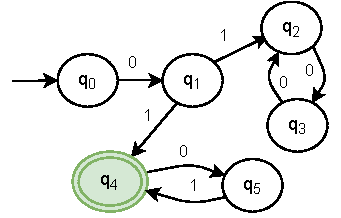
\includegraphics[]{diagrams-Original A.pdf}
	\caption{Non-deterministic finite automaton $A_1$.}
	\label{fig:NFA_A1_orig}
\end{figure}

$A_1$ is a non-deterministic finite automaton (see state $q_1$) and uses multiple input symbols. Due to the fact we work with only recognized word lengths, we can substitute the automaton alphabet with a unary alphabet of a single input symbol $*$\footnote{Even though we do not actually need any particular input symbol, we use \emph{*} here as an example to depict the process. In general, all we need to know is that there is a transition between two states. The specific transition symbols are not significant for our length abstraction.}. See the obtained finite automaton $A'_1$ in Figure~\ref{fig:NFA_A1_star}.

\begin{figure}[ht]
	\centering
	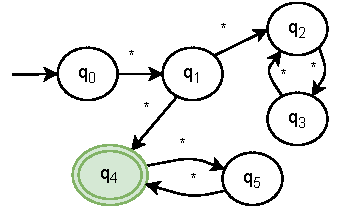
\includegraphics[]{diagrams-Original A Star.pdf}
	\caption{Non-deterministic finite automaton $A'_1$: $A_1$ with unified transition symbols.}
	\label{fig:NFA_A1_star}
\end{figure}

Then, we can generate \LSAa{$q_0$}, which is its deterministic equivalent. For the final \LSAa{$q_0$}, generated from $A'_1$ by its product construction determinization, see Figure~\ref{fig:HaL_A1}. Lasso automaton for $q_0$ accepts any words of lengths of words recognized by state language of $q_0$.

\begin{figure}[ht]
	\centering
	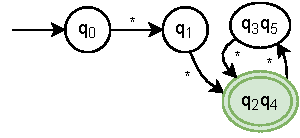
\includegraphics[]{diagrams-lsa-q0.pdf}
	\caption{Lasso automaton \LSAa{$q_0$} for the original NFA $A_1$ generated from $A'_1$ by its determination with subset construction.}
	\label{fig:HaL_A1}
\end{figure}

%--------------------------------------------------------
%--------------------------------------------------------
\subsection{Single Lasso Automaton for Each Original Automaton}\label{sec:singleHaL}

When we are constructing a product of finite automata $A$ and $B$, we do not want to regenerate $\LSAa{q_A}$ and $\LSAa{q_B}$ for each product state $p = [q_A, q_B]$. This is inefficient. Due to the nature of LSAs, the successive product states $p' = [q'_A, q'_B]$ generate LSAs very similar to the LSAs for $p$. We can construct one summary lasso automaton for the whole finite automaton $A$, $\LSAA{A}$, which contains all the lasso automata $\LSAa{q_A}$ for all states in $A$. Similarly for $B$.

$\LSAA{A}$ is a lasso automaton created as a union of all $\LSAa{q_A}$ for each $q_A \in Q_A$. That is, $\LSAA{A}$ is a union of all lasso states, transitions, final and initial states for each $q_A$. As a result, $\alpha^{LA}$ for product construction generates only one LSA for each finite automaton (possibly with multiple loops and/or multiple handles). All singleton states in $\LSAA{A}$ can be initial states. The initial state changes to which state $q_A$ we want $\LSAa{q_A}$ for.

To generate only the necessary $\LSAa{q_A}$, we can construct $\LSAA{A}$ gradually, state by state, for only the currently required $q_A$. We generate $\LSAa{q_A}$ as the first part of $\LSAA{A}$. If we need $\LSAa{q'_A}$ later, we extend $\LSAa{q_A}$ with $\LSAa{q'_A}$ by union of both LSAs. When the new LSA state $l_A$ is not already present in $\LSAA{A}$, we add $l_A$ to $\LSAA{A}$ and continue with the following states $l'_A$ until we either create an entirely new loop in $\LSAA{A}$ or generate $l'_A$ already in $\LSAA{A}$ (we can stop generating $l'_A$ as from now on, all $l'_A$ are already in $\LSAA{A}$.

By executing the same steps for $B$, we get two LSAs, one for each finite automaton.

\paragraph{Running Example}

For our finite automaton $A_1$, Figure~\ref{fig:NFA_A1_LSA_A} shows $\LSAA{A_1}$, currently prepared for an extraction of the length formulae for $q_0$. However, the initial state is irrelevant for the general $\LSAA{A_1}$, as it changes to the state we are currently computing length abstraction formulae for.

\begin{figure}[ht]
	\centering
	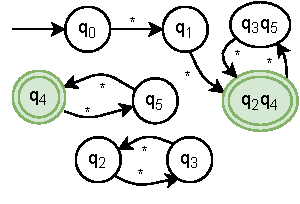
\includegraphics[]{diagrams-LSA-A.pdf}
	\caption{Summary lasso automaton $\LSAA{A_1}$.}
	\label{fig:NFA_A1_LSA_A}
\end{figure}

%--------------------------------------------------------
%--------------------------------------------------------
\subsection{Product Construction with Length Abstraction}

The core of the product construction remains unchanged, but there are a few differences. The Algorithm~\ref{productConstructionLengthAbstrAlg} shows how we alternate the original product construction to optimize the algorithm with length abstraction.

\begin{algorithm}[ht]
\caption{Product construction with length abstraction.}\label{productConstructionLengthAbstrAlg}
\SetKwInOut{Input}{Input}\SetKwInOut{Output}{Output}
\DontPrintSemicolon
\Input{ NFA $A_1 = (Q_1, \Sigma, \delta_1, I_1, F_1)$, NFA $A_2 = (Q_2, \Sigma, \delta_2, I_2, F_2)$}
\Output{ NFA $P = (A_1 \cap A_2) = (Q, \Sigma, \delta, I, F)$ with $L(P) = L(A_1) \cap L(A_2)$}
\BlankLine
$Q, \delta, F \gets \emptyset$ \;
$I \gets I_1 \times I_2$ \;
$W \gets I$ \;\label{work_set}
$res \gets False$ \;\label{sat}
$solved \gets \emptyset$ \;\label{solved}
\While{$W \neq \emptyset$}{
    \textbf{picklast} $[q_1, q_2]$ \textbf{from} $W$\label{picklast} \;
    \textbf{add} $[q_1, q_2]$ \textbf{to} $solved$ \;
    $res \gets \abstLA{q_1} \land \abstLA{q_2} \textbf{ is } \emph{sat}$\label{satisfiable} \;
    \If{$res = True$}{\label{AlgSolveForSat}\label{satTrue}
        \textbf{add} $[q_1, q_2]$ \textbf{to} $Q$ \;
        \If{$q_1 \in F_1$ \textbf{and} $q_2 \in F_2$} {
        \textbf{add} $[q_1, q_2]$ \textbf{to} $F$ \;
        }\label{AlgAddToFinalState}
        \ForAll{$a \in \Sigma$}{
            \ForAll{$q'_1 \in \delta_1(q_1, a), q'_2 \in \delta_2(q_2, a)$}{
                \If{$[q'_1, q'_2] \notin solved$ \textbf{and} $[q'_1, q'_2] \notin W$}{
                    \textbf{add} $[q'_1, q'_2]$ \textbf{to} $W$ \;
                }
                \textbf{add} $[q'_1, q'_2] \textbf{ to } \delta([q_1, q_2], a)$ \;
            }
        }
    }
}
\end{algorithm}

We call $W$ from line \ref{work_set} a work set. It stores the potential product states prepared for processing, which we pick from $W$ one by one\footnote{In spite of the fact more approaches are valid, we strongly recommend picking the last added product state from $W$ (see line \ref{picklast})---using depth-first search---as this allows us to quickly advance through the automaton and get to any final state faster---in case we just want to know whether automata have a non-empty intersection, this change will get us the answer most of the time in less steps. It works even better when implemented with a satisfiable state skipping optimization, explained in Section~\ref{sec:skipping states}.}.

The optimization process starts when we pick a product state $p$ from $W$. Instead of immediately generating new successive product states $p'$, we generate $\LSAa{q_1}$ and $\LSAa{q_2}$ to gain length formula. We test the satisfiability of this formula: $\sat{\compatLA{p}}$ where
\[
    \compatLA{p} : \abstLA{q_1} \wedge \abstLA{q_2} \text{ and}
\]
$\sat{\psi}$ is \emph{True} iff $\psi$ is satisfiable ($\Phi \textbf{ is } \emph{sat}$), $False$ otherwise. On line \ref{satisfiable}, we check whether $\sat{\compatLA{p}}$ holds and store a result as a boolean value to $res$. We are only interested in the satisfiability test result because we do not need any additional information from the computed formulae. Therefore, a simple boolean value is sufficient. $\compatLA{p}$ is passed to an SMT solver to solve its satisfiability. The $\alpha^{LA}$ compatibility check $ \abstLA{q_1} \land \abstLA{q_2} \textbf{ is } \emph{sat}$ can be implemented in SMT solver as in Algorithm~\ref{checkLengthAbstractionSatisfiabilitySMTAlgorithm}. SMT solver returns \emph{sat} when satisfiable ($res$ is set to \emph{True}) and \emph{unsat} when unsatisfiable ($res$ is set to \emph{False}). If \emph{unsat} is returned, length abstractions are incompatible. We have now pruned the generated state space by omitting the product state $p$.

\begin{algorithm}[ht]
\newcommand{\LAFormula}[1]{\varphi_{#1}}

\caption{Check compatibility of length abstractions with SMT solver.}\label{checkLengthAbstractionSatisfiabilitySMTAlgorithm}
\SetKwInput{Input}{Input}
\SetKwInput{Output}{Output}
\SetKw{Return}{return}
\SetKw{Break}{break}
\SetKwFunction{FIsLengthAbstractionSatisfiable}{isLengthAbstractionSatisfiable}
\SetKwFunction{FSMTInit}{smtInit}
\SetKwFunction{FSMTAdd}{smtAdd}
\SetKwFunction{FSMTPush}{smtPush}
\SetKwFunction{FSMTPop}{smtPop}
\SetKwFunction{FSMTCheck}{smtCheck}
\SetKwProg{Fn}{Function}{:}{}

\DontPrintSemicolon
\BlankLine

$\FSMTInit{}$ \;
$\FSMTAdd{$k \geq 0, m \geq 0$}$ \;

\For{$\LAFormula{q_1} \in \abstLA{q_1}$}{
    \For{$\LAFormula{q_2} \in \abstLA{q_2}$}{
        $\FSMTPush{}$ \;
        $\FSMTAdd{$\LAFormula{q_1}.handle + \LAFormula{q_1}.lasso * k = \LAFormula{q_2}.handle + \LAFormula{q_2}.lasso * m$}$ \;
        $res \gets \FSMTCheck{}$ \;
        \If{$res = True$}{
            \Break \;
        }
        $\FSMTPop{}$ \;
    }
}
\end{algorithm}

If $\sat{\compatLA{p}}$, i.e., there will be an accepting run using $p$ (see line \ref{satTrue}), we add $p$ to $Q$, possibly to $F$ and generate $p'$.

A note of caution. It is important to understand that we are working only with possible word lengths and when we test the emptiness of the intersection of automata, we can resolve only such cases where words lengths are not accepted by both automata. When the test shows there could be some words of certain length accepted by both automata and for that reason by their intersection too---$\sat{\compatLA{p}}$---we cannot be sure there truly are any words accepted by both automata with their intersection non-empty, because there may be words of the suggested length, but it may be a different word for each automaton (which differ from one another in the containing symbols or their position in the word). For resolving such cases, we have to proceed with the classic algorithm steps to produce product states according to their original transition symbols, not only by comparing the possible words lengths. With certainty, we can omit only the cases where $\neg \sat{\compatLA{p}}$.

\paragraph{Running Example}

We will continue with our running example. The second automaton we will be working with is a NFA $A_2 = (\{s_0, s_1, s_2, s_3\}, \{0, 1\}, \delta_2, \{s_0\}, \{s_3\}) $ where $\delta_2$ is depicted in Figure~\ref{fig:NFA_A2_orig}.

\begin{figure}[ht]
    \centering
	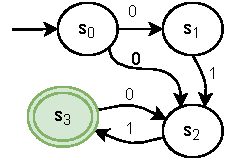
\includegraphics[]{diagrams-Original B.pdf}
	\caption{Non-deterministic finite automaton $A_2$.}
	\label{fig:NFA_A2_orig}
\end{figure}

In Figure~\ref{fig:HaL_A2}, there is \LSAA{$A_2$}, which we will be using together with \LSAA{$A_1$} shown in Figure~\ref{fig:NFA_A1_LSA_A} for product construction of $A_1$ and $A_2$.

\begin{figure}[ht]
    \centering
	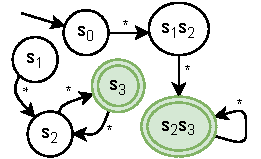
\includegraphics[]{diagrams-Final Handle and Loop Automaton B.pdf}
	\caption{Lasso automaton \LSAA{$A_2$} for $A_2$.}
	\label{fig:HaL_A2}
\end{figure}

When we start the algorithm, we get the following length abstraction formulae for $p = [q_0, s_0]$. From \LSAA{$A_1$} for $q_0$ ($q_0$ is the new initial state of $\LSAA{A_1}$), we get an existential formula representing length abstraction $\abstLA{q_0}$\footnote{This formula consists of two independent disjuncts $\varphi_1$ and $\varphi_2$ describing there are more possible lengths for accepted words from the same initial state.}. From \LSAA{$A_2$} for $s_0$ ($s_0$ is the new initial state of $\LSAA{A_2}$), we get a formula for length abstraction $\abstLA{s_0}$\footnote{We are using variable $m$ here instead of $k$ to emphasize variables from different formulae are not dependent on each other---they belong to different LSAs.}.
\begin{align*}
    &\abstLA{q_0}: \exists k ( |w| = 2 \lor |w| = 4 + 2 \cdot k ) \\
    &\abstLA{s_0}: \exists m ( |w| = 2 + 1 \cdot m )
\end{align*}

When we compare $\abstLA{q_0}$ and $\abstLA{s_0}$, we get:
\[
    \abstLA{q_0} \land \abstLA{s_0} : \exists k ( |w| = 2 \lor |w| = 4 + 2 \cdot k ) \land \exists m ( |w| = 2 + 1 \cdot m )
\]
or in a simplified notation:
$$ \abstLA{q_0} \land \abstLA{s_0} : \exists k \exists m ( 2 \lor 4 + 2 \cdot k = 2 + 1 \cdot m ) \text{.} $$

To solve satisfiability of $\compatLA{[q_0, s_0]}$, we try to find values of $k$ and $m$ such that $|w|$ in both formulae are equal (some expressions on the left and on the right side of the equation are equal).

In Figure~\ref{fig:product_WIP}, we can see the product of $A_1$ and $A_2$ being constructed using length abstraction. Red states represent product states whose formulae are resolved as unsatisfiable and therefore the algorithm omits any successive product states---dashed states (such as $q_4s_2$ or $q_3s_2$) which are generated in the unoptimized product construction. The green state represents final states in both automata. Here, we have found a solution accepted by both $A_1$ and $A_2$. If we desire to resolve only the emptiness problem, we can stop the execution of the algorithm here as we have found one final state---automata have non-empty intersection. The blue state is a normal product state whose significance will be explained in section~\ref{sec:skipping states}.

\begin{figure}[ht]
	\centering
	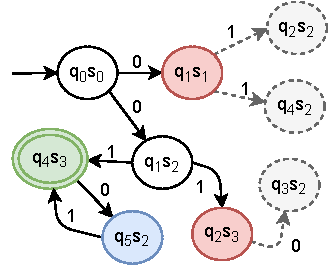
\includegraphics[]{diagrams-skip WIP Product .pdf}
	\caption{Constructed product with depiction of optimization with length abstraction.}
	\label{fig:product_WIP}
\end{figure}

As you can notice in Figure~\ref{fig:product_final}, the product generated by our algorithm has only 4 product states in comparison to 9 product states generated by the unoptimized product construction.

\begin{figure}[ht]
	\centering
	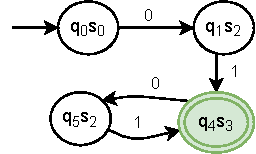
\includegraphics[]{diagrams-Final Product.pdf}
	\caption{Final product minimized by length abstraction.}
	\label{fig:product_final}
\end{figure}

%--------------------------------------------------------
%--------------------------------------------------------

\subsection{Optimization with Skipping Satisfiable States} \label{sec:skipping states}

When we take new $p$ from $W$ and $\sat{\compatLA{p}}$, it is time to add all the possible successive product states $p'$ to $W$. When $p$ generates only a single $p'$ and $p \not \in F_P$ (final states are obviously in the product) or satisfiable length was not zero\footnote{If the satisfiable length is zero, we are in a final product state and $p$ generated from final state might not lead to any final state, but the length abstractions for final state are compatible, of course.}, we can say with certainty that $\sat{\compatLA{p'}}$ as there is only a single branch in the automaton leading from $p$ to a~final state (through $p'$). $p'$ is \emph{skippable}, iff there exists $p \not \in F_P$ or with satisfiable length not zero for which $\sat{\compatLA{p}}$ and whose only successor is $p'$, we add $p'$ to $W$ with the information of being skippable. If $p'$ is already in~$W$, we append the information to $p'$ in $W$.

We skip checking for $\sat{\compatLA{p'}}$ when we pick $p'$ from $W$. We can immediately check for final states and generate the successive product states. This optimization saves us generating the length abstraction formulae for $p'$ and testing the formulae in the SMT solver for their satisfiability.

If automata have long lines (with non-splitting branches), this will prove extremely useful, because only a few proper iterations with formulae computing and running SMT solver computation will be executed. The application of skipping satisfiable states is depicted in Algorithm~\ref{productConstructionLengthAbstrAlgSkip}. The line~\ref{satisfiable} from Algorithm~\ref{productConstructionLengthAbstrAlg} is substituted with the contents of Algorithm~\ref{productConstructionLengthAbstrAlgSkip}.

%{ \LinesNotNumbered
\begin{algorithm}[ht]
\SetKwFunction{FSkippable}{skippable}
\SetKwFunction{FSatisfiable}{satisfiable}
    \caption{Substitution of line~\ref{satisfiable} in Algorithm~\ref{productConstructionLengthAbstrAlg} with skipping satisfiable states.} \label{productConstructionLengthAbstrAlgSkip}
    \DontPrintSemicolon
    \eIf{$ \FSkippable{$[q_1, q_2]$}$}{
        $res \gets True$ \;
    }{
        $res \gets \abstLA{q_1} \land \abstLA{q_2} \textbf{ is } \emph{sat}$ \;
    }
\end{algorithm}
%}

The only change is a test for every checked $p$, which decides whether $p$ can be skipped. You can see that we proceed with the satisfiability check in SMT solver only for $p$ which are generated from the product states with multiple transitions generating $p$ and at least one more product state (in general at least two new potential product states). If only one $p$ was generated earlier from a product state with satisfiable formulae, we skip the check for $\sat{\compatLA{p}}$ and continue to generating its successive states immediately.

You can notice there is one skippable state in the former example, which had to be evaluated and tested for satisfiability earlier. The blue state in Figure~\ref{fig:product_WIP} is such a skippable state. In our case for state $q_5s_2$, when only one new state is generated from state $q_4s_3$ while this state is resolved as satisfiable (with not zero length---otherwise, if $q_5s_2$ did not lead back to $q_4s_3$, $q_5s_2$ would be skippable even though it would not lead to any final state), newly generated product state has to be satisfiable as well, because the check for $q_4s_3$ already considered the state $q_5s_2$ as its only way to any final state with not zero length.

When we have a series of such states, we can highly optimize generating the whole branch with only one initial check for satisfiability. In real world examples, there are often automata with long branches splitting into multiple branches only occasionally. We will check for satisfiability for all the initial states of each new branch and then either omit the entire branch (if \emph{unsat} is returned) or skip checking satisfiability in the entire branch (if \emph{sat} is returned).

\subsection{Resolving Length Abstraction Satisfiability without SMT Solver}

Evaluating satisfiability of length abstractions formulae in SMT solver is expensive. We try to replace SMT solver with a specialized structure which transforms the problem of solving satisfiability of length abstraction formulae to evaluating satisfiability of a linear congruence equations.

Length abstraction formulae have the same, simple structure. Length abstraction can be implemented as a set of length formulae represented as a two-tuple of handle length and lasso length. Therefore, we can easily compare such sets in order to resolve satisfiability of length abstraction formulae without SMT solver. $\compatLA{p}$ forms a set of linear congruence equations, which can be resolved just by utilizing basic mathematical operations and properties of linear congruences.

The Algorithm~\ref{checkLengthAbstractionSatisfiabilitySMTFreeAlgorithm} shows how to determine $\sat{\compatLA{p}}$ from line~\ref{satisfiable} using linear congruences.

\begin{algorithm}[ht]
\newcommand{\LAFormula}[1]{\varphi_{#1}}

\caption{Check satisfiability using length abstraction algorithm without SMT solver.}\label{checkLengthAbstractionSatisfiabilitySMTFreeAlgorithm}
\SetKw{Return}{return}
\SetKwFunction{FIsLengthAbstractionSatisfiable}{isLengthAbstractionSatisfiable}
\SetKwFunction{FSolveForOneHandleLonger}{solveForOneHandleLonger}
\SetKwFunction{FGetGCD}{getGCD}
\SetKwProg{Fn}{Function}{:}{}

\DontPrintSemicolon
% The function code itself.
\For{$\LAFormula{q_1} \in \abstLA{q_1}$}{
    \For{$\LAFormula{q_2} \in \abstLA{q_2}$}{
        \uIf{$\LAFormula{q_1}.handle = \LAFormula{q_2}.handle$}{
            $res \gets True$ \;
        } \uElseIf{$\LAFormula{q_1}.handle > \LAFormula{q_2}.handle$}{
            $res \gets \FSolveForOneHandleLonger{$\LAFormula{q_1}$, $\LAFormula{q_2}$}$ \;
        } \uElse{
            $res \gets \FSolveForOneHandleLonger{$\LAFormula{q_2}$, $\LAFormula{q_1}$}$ \;
        }
    }
}

$res \gets False$ \;
\end{algorithm}

We execute the following steps for each equation
\[
    \varphi_{q_1}.handle + \varphi_{q_1}.lasso \cdot k = \varphi_{q_2}.handle + \varphi_{q_2}.lasso \cdot m \text{.}
\]

If the handle lengths of $\varphi_{q_1}$ and $\varphi_{q_2}$ are equal, there are words of the same length accepted by both $\abstLA{q_1}$ and $\abstLA{q_2}$ (they are mutually compatible) without stepping into the loops of \LSAA{$A_1$} and \LSAA{$A_2$}. Otherwise, handle lengths differ, and we must consider lengths of loops in our determination of compatibility of $\abstLA{q_1}$ and $\abstLA{q_2}$.

We now have to determine $\sat{\varphi_{q_1} \land \varphi_{q_2}}$ for abstractions with one handle longer. This is solved by the function \texttt{solveForOneHandleLonger} in Algorithm~\ref{checkLengthAbstractionSatisfiabilitySMTFreeAlgorithmFunctionImplementation}.

\begin{algorithm}[ht]
\newcommand{\LAFormulaLonger}{\varphi_{l}}
\newcommand{\LAFormulaShorter}{\varphi_{s}}
\newcommand{\HandleDifference}{\LAFormulaLonger.handle}
\newcommand{\CurrentIteration}{it}

\caption{Solve satisfiability of length abstraction formulae for one handle longer.}\label{checkLengthAbstractionSatisfiabilitySMTFreeAlgorithmFunctionImplementation}
\SetKw{Return}{return}
\SetKwFunction{FIsLengthAbstractionSatisfiable}{isLengthAbstractionSatisfiable}
\SetKwFunction{FSolveForOneHandleLonger}{solveForOneHandleLonger}
\SetKwFunction{FGetGCD}{getGCD}
\SetKwProg{Fn}{Function}{:}{}

\DontPrintSemicolon
\Fn{\FSolveForOneHandleLonger{$\LAFormulaLonger$, $\LAFormulaShorter$}}{
    \KwData{
    Input length abstraction formulae of potential product state.\\
    $\LAFormulaLonger$: Length abstraction formula with the longer handle, \\
    $\LAFormulaShorter$: Length abstraction formula with the shorter handle.
    }
    \KwResult{bool: \emph{True} if satisfiable, \emph{False} otherwise.}

    % The function code itself.
    $\HandleDifference \gets \LAFormulaLonger.handle - \LAFormulaShorter.handle$ \label{simplifyEquation} \;
    $\LAFormulaShorter.handle \gets 0$ \;

    \uIf{$\LAFormulaLonger.lasso = 0 \textbf{ and } \LAFormulaShorter.lasso = 0$}{\label{both_no_loops}
        \Return $False$ \;
    } \uElseIf{$\LAFormulaShorter.lasso = 0$}{\label{shorter_no_loop}
        \Return $False$ \;
    } \uElseIf{$\LAFormulaLonger.lasso = 0$}{\label{longer_no_loop}
        $\CurrentIteration \gets 0$ \tcp*[h]{Current length resembling the iteration of the shorter lasso loop.} \;
        \While{$\CurrentIteration \leq \HandleDifference$}{
            \eIf{$\CurrentIteration = \HandleDifference$}{
                \Return $True$ \;
            }{
                $\CurrentIteration \gets \CurrentIteration + \LAFormulaShorter.lasso$ \;
            }
        }
        \Return $False$ \;
    } \uElse{\label{both_loops}
        $gcd \gets \FGetGCD{$\LAFormulaLonger.lasso$, $\LAFormulaShorter.lasso$}$ \;
        \eIf{$gcd = 1$}{
            \Return $True$ \;
        }{
            $y \gets - \HandleDifference$ \;
            \While{$y < gcd$}{
                $y \gets y + \LAFormulaShorter.lasso$ \;
            }
            \eIf{$(y \mod gcd) = 0$}{
                \Return $True$ \;
            } {
                \Return $False$ \;
            }
        }
    }
}
\end{algorithm}

First, to simplify the equation (line~\ref{simplifyEquation}), we move handle lengths from the side of the equation with the shorter handle $\varphi_s$ to the side with the longer handle $\varphi_l$ to solve:
\begin{equation}\label{simplified_equation}
    \varphi_{l}.handle + \varphi_{l}.lasso \cdot k = \varphi_{s}.lasso \cdot m
\end{equation}
which represents the number of loops a word must make in $\varphi_{s}$ to be accepted by $\varphi_l$ (as if with shorter $\varphi_l.handle$).

If both $\varphi_l$ and $\varphi_s$ have no loops (line~\ref{both_no_loops}), $\varphi_{q_1} \land \varphi_{q_2}$ is unsatisfiable because the handles differ. Else, if only $\varphi_s$ has no loop (line~\ref{shorter_no_loop}), every word accepted by $\varphi_s$ is shorter than words accepted by $\varphi_l$ and the formulae cannot be satisfiable.

Else, if only $\varphi_l$ has no loop (line~\ref{longer_no_loop}), we can try to manually iterate over loops in $\varphi_s$ to see whether the difference of word lengths between handles can be equalized by looping in $\varphi_s.lasso$.

Otherwise, both $\varphi_l$ and $\varphi_s$ have loops (line~\ref{both_loops}). We can apply linear congruence properties to the equation~\ref{simplified_equation} to determine whether the formulae are satisfiable. The equation~\ref{simplified_equation} says that if formulae are satisfiable, the left side of the equation is divisible by some multiple of $\varphi_s.lasso$. We can rewrite that in a linear congruence equation as follows:
\begin{align}
    \varphi_{l}.handle + \varphi_{l}.lasso \cdot k &\equiv 0 \pmod{\varphi_s.lasso} \\
    \varphi_{l}.lasso \cdot k &\equiv - \varphi_{l}.handle  \pmod{\varphi_s.lasso} \label{linear_congruence_equation}
\end{align}
which is the same as solving a linear Diophantine equation
\begin{equation}
    \varphi_{l}.lasso \cdot k - \varphi_s.lasso \cdot m = - \varphi_{l}.handle \text{.} \label{linear_diophantine_equation}
\end{equation}

Properties of multiplicative inverse~\cite{DivisibilityAndGreatestCommonDiviser, LinearCongruences}, based on Bézout's identity~\cite{DivisibilityAndGreatestCommonDiviser}, say that iff $\varphi_l.lasso$ and $\varphi_s.lasso$ are relatively prime (coprime)---the greatest common divisor (GCD) of $\varphi_l.lasso$ and $\varphi_s.lasso$ is equal to $1$---there exists a multiplicative inverse for $\varphi_l.lasso$ in modulo $\varphi_s.lasso$ which ensures that linear congruence~\ref{linear_congruence_equation} is always solvable for some $\varphi_l.lasso$ in modulo $\varphi_s.lasso$\footnote{We can get the precise solution by multiplying both sides of the equation with the multiplicative inverse.}. Therefore, the formulae are satisfiable.

Otherwise, $\varphi_l.lasso$ and $\varphi_s.lasso$ are not coprime (GCD is different from $1$) and by properties of linear Diophantine equations~\cite{LinearCongruences}, iff GCD precisely divides $y$ without a remainder where $y$ is the right side of the linear congruence~\ref{linear_congruence_equation} or its any congruent equivalent, there exist solutions to the linear congruence\footnote{We can apply extended Euclidean algorithm to find the precise values for the Diophantine equation~\ref{linear_diophantine_equation}.}. Otherwise, there are no solutions.

%--------------------------------------------------------
%--------------------------------------------------------
%--------------------------------------------------------
%--------------------------------------------------------
\section{Parikh Image Abstraction of State Languages}

Length abstraction is a simple and fast optimization, but can be too coarse to detect non-terminating states in some cases. In this section, we present an abstraction of state languages with Parikh images, $\alpha^{PI}$, which aims to replace length abstraction to make the abstraction more precise to prune larger quantities of product state space.

Parikh images provide more information about the finite automata than simple length abstraction. While length abstraction considers only accepted word lengths without knowing which transition symbols are actually in the transitions, Parikh image abstracts the state language to numbers of occurrences of specific transition symbols in words regardless of their position in said words. Thus, Parikh image abstraction allows us to more precisely determine whether the product state has non-empty language. However, Parikh image computation itself is expensive. The question is, whether the added computation time compensates for more precise product generation with higher state pruning capabilities.

We will introduce an algorithm for Parikh image abstraction $\alpha^{PI}$ applied on each product state $p = [q_1, q_2]$ to decide the compatibility of $\abstPI{q_1}$ and $\abstPI{q_2}$.

\subsection{Parikh Image} \label{sec:parikhImage}

We derive our Parikh image construction from the Parikh's theorem~\cite{Kozen1977} described in~\cite{ParikhsTheoremSimpleAndDirectConstruction}, creating a semi-linear Parikh image formulae for the given regular language as a set of Parikh images for each word in the language. However, our usage of Parikh image of some regular language (and therefore of the corresponding finite automaton recognizing such regular language) is restricted to determining the compatibility of Parikh image state language abstractions. Therefore, we only test for satisfiability of Parikh image formulae describing $\abstPI{q}$. We use SMT solver to resolve the satisfiability of Parikh image formulae of the current potential product state.

% where $I$ is a singleton $I = \{ q_{0} \}$
Given an NFA $A = (Q, \Sigma, \Delta, I, F)$, Parikh image formula $\varphi$ (as described in~\cite{PI_computation/10.1007/978-3-030-45093-9_59} for solving string constraints) consists of several constraints in conjunctive normal form. $\varphi$ describes runs of $A$. Each satisfiable assignment defines properties of the run. $\varphi$ consists of the following conjuncts:

\begin{enumerate}
    \item \label{clauses:u_original} Foremost, we define a variable $u_{q}$ for each state $q \in Q$. $u_{q}$ defines how many times we enter $q$ and exit $q$ by specifying the difference between the number of entries and exits. We construct equations with $u_{q}$ for a run as follows:
    \begin{itemize}
        \item $u_{q} = 1$ for $q \in I$,
        \item $u_{q} \in \{ 0, -1 \}$ for $q \in F$ and
        \item $u_{q} = 0$ for $q \in Q \setminus ( I \cup F )$.
    \end{itemize}

    \item \label{clauses:y_original} Second, we define a variable $y_{t}$ for each transition $t \in \Delta$ such that $y_{t} \geq 0$ describing how many times is $t$ used in the run.

    \item \label{clauses:uy_original} We can now present an equation introducing a connection between $u_{q}$ and $y_{t}$ to evaluate the difference between the number of entries and exits for each $q \in Q$ as follows:
    $$ u_q + \sum_{t \in \Delta_q^+} y_t - \sum_{t \in \Delta_q^-} y_t = 0.$$
    where $\Delta_q^+$ is a set of ingoing transitions $ \Delta_q^+ = \{ (q',a,q) \in \Delta \}$ and $\Delta_q^-$ is a set of outgoing transitions $ \Delta_q^- = \{ (q,a,q') \in \Delta \} $ from the given state $q$.

    \item \label{clauses:z_original} Furthermore, we need to make sure that the states used in runs described by the satisfying assignments are connected and start in the initial state. Variable $z_q$ for each $q \in Q$ is introduced. $z_q$ represents the length of any path from $I$ to $q$ in a spanning tree of the subgraph with $y_t \geq 0$. If $z_q = 0$, there is no path from $I$ to $q$ and the state $q$ is not used in the run. $z_q > 0$ means there is a path from $I$ to $q$ and $q$ is used in the run.

    If $q \in I$, we add a constraint $z_q = 1 \land y_t \geq 0$. Otherwise,
    {
    \begin{align*}
        (z_q = 0 \land \bigwedge_{t \in \Delta_q^+} y_t = 0) \lor \bigvee_{t \in \Delta_q^+} (y_t \geq 0 \land z_{q'} \geq 0 \land z_q = z_{q'} + 1) \text{.}
    \end{align*}
    }
    If the distance $z_q$ is $0$, $q$ is not in the run.

    \item \label{clauses:hash_original} Last but not least, we declare the only free variable $\#_a$ for each transition symbol $ a \in \Sigma$. $\#_a$ describes the number of occurrences of $a$ in accepted words regardless of their position in the words (the number of $a$ in the run). $\#_a$ is the only variable common to different Parikh image abstractions when we test their compatibility. The constraint $\#_a = \sum_{t = (q, a, q') \in \Delta} y_t$ ensures $\#_a$ is consistent with the number of used $t$ with $a$.

\end{enumerate}

We gain an existentially quantified formula $\varphi$ in Presburger arithmetic describing language abstracting $\alpha^{PI}$ for $A$ with free variables $\#_a$:
$$ \alpha^{PI} : \exists u_{q_1},\ldots,u_{q_n},z_{q_1},\ldots,z_{q_n},y_{t_1},\ldots,y_{t_m} ( \varphi ) $$
where $n = \lvert Q \rvert$ is the number of states and $m = \lvert \Delta \rvert$ is the number of transitions in the finite automaton.

Notice that $\alpha^{PI}$ is an existential formula, which is great for SMT solving where computing with universal quantifiers can take a long time. SMT solver are specialized on efficient solving of existential or quantifier-free formulae.

As for length abstraction for product state $p = [q_1, q_2]$, we decide compatibility of Parikh image formulae $\abstPI{q_1}$ and $\abstPI{q_2}$ as follows: $\sat{\compatPI{p}}$ such that
\[
    \compatPI{p} : \abstPI{q_1} \wedge \abstPI{q_2}\footnotemark \text{.}
\]
\footnotetext{In reference implementation, we replace existential formulae with quantifier-free formulae with renamed variables without existential quantifiers.}

\subsection{Product Construction with Parikh Image Abstraction}

We introduce the unoptimized product construction using Parikh image abstraction. The algorithm is analogous to the product construction optimized by length abstraction from Algorithm~\ref{productConstructionLengthAbstrAlg}. The difference is that we now compute Parikh image formulae and determine their satisfiability instead of generating lasso automata and determining satisfiability of length abstraction formulae.

We use Parikh image formulae to determine whether $p$ is to be added to the product~$P$. As for length abstraction, we test whether Parikh image abstractions are compatible (a conjunction of Parikh image formulae is satisfiable). Therefore, instead of length abstraction on line~\ref{satisfiable} in Algorithm~\ref{productConstructionLengthAbstrAlg}, we compute Parikh image abstractions: line~\ref{satisfiable}  is replaced with
\[
    res \gets \abstPI{q_1} \land \abstPI{q_2} \textbf{ is } sat
\]

We can see our proposed algorithm using Parikh image computation to optimize product construction in the Algorithm~\ref{productConstructionParikhImageAlgorithm}. Parikh image formulae are computed on line~\ref{areParikhImageFormulaeSatisfiable} and their satisfiability is determined.

\begin{algorithm}
\caption{Product construction with Parikh image abstraction.}\label{productConstructionParikhImageAlgorithm}
\SetKwInOut{Input}{Input}
\SetKwInOut{Output}{Output}
\SetKwFunction{FStateAbstractionPI}{$ \alpha^{PI} $}
\DontPrintSemicolon
\Input{ NFA $A_1 = (Q_1, \Sigma, \delta_1, I_1, F_1)$, NFA $A_2 = (Q_2, \Sigma, \delta_2, I_2, F_2)$}
\Output{ NFA $P = (A_1 \cap A_2) = (Q, \Sigma, \delta, I, F)$ with $L(P) = L(A_1) \cap L(A_2)$}
\BlankLine
$Q, \delta, F \gets \emptyset$ \;
$I \gets I_1 \times I_2$ \;
$W \gets I$ \;
$res \gets False$ \;
$solved \gets \emptyset$ \;\label{PIAlgorithm:solved}
\While{$W \neq \emptyset$}{\label{PIAlgorithm:IterateOverProductStates}
    \textbf{picklast} $[q_1, q_2]$ \textbf{from} $W$ \;
    \textbf{add} $[q_1, q_2]$ \textbf{to} $solved$ \;

    $res \gets \FStateAbstractionPI{$q_{1}$} \land \FStateAbstractionPI{$q_{2}$} \textbf{ is } \emph{sat} $ \label{areParikhImageFormulaeSatisfiable} \;

    \If{$res = True$}{
        \textbf{add} $[q_1, q_2]$ \textbf{to} $Q$ \;
        \If{$q_1 \in F_1$ \textbf{and} $q_2 \in F_2$} {
        \textbf{add} $[q_1, q_2]$ \textbf{to} $F$ \;
        }
        \ForAll{$a \in \Sigma$}{
            \ForAll{$q'_1 \in \delta_1(q_1, a), q'_2 \in \delta_2(q_2, a)$}{
                \If{$[q'_1, q'_2] \notin solved$ \textbf{and} $[q'_1, q'_2] \notin W$}{
                    \textbf{add} $[q'_1, q'_2]$ \textbf{to} $W$ \;
                }
                \textbf{add} $[q'_1, q'_2] \textbf{ to } \delta([q_1, q_2], a)$ \;
            }
        }
    }
}
\end{algorithm}

\subsection{Reduced Parikh Image}\label{sec:reducedParikhImage}

The presented Parikh image would work well regarding its pruning capabilities. However, the described Parikh image computation requires extensive resources and computation time and we need Parikh images computed only for determining the emptiness of the intersection. Given that most of the computation time is spent by the evaluation of Parikh image conjuncts in SMT solver, we want to minimize the number of Parikh image conjuncts SMT solver needs to evaluate for each $\varphi$.

Consequently, we infer our reduced Parikh image from the shown Parikh image to further optimize Parikh image computation. We modify several conjuncts in Parikh image formula and unify initial states and accepting states to simplify the formula and reduce its complexity.

Due to how we have reduced our Parikh image, we work only with finite automata with a single initial state and a single accepting state. However, we can easily convert any finite automaton into the required format with adding two new states: one for a new initial state from which one can transition to all previous initial states and one for a new accepting state to which lead all previous accepting states. The previous initial and accepting states are changed to common automata states.


%TODO Unification of inital and accepting states

Our reduced Parikh image consists of the following conjuncts:
\begin{enumerate}
    \item \label{clauses:u_reduced} We use the conjuncts~\ref{clauses:u_original}, except now we restrict $u_q$ for each final state to have only the value $-1$, i.e.:
    $$ u_{q} = -1 \text{ for each state } q \in F \text{.}$$

    We can perform this reduction, because we know for sure that by unifying final states of the automaton into one abstract final state, there will be exactly only one final state where all words accepted by the automaton end, but none passes through this state earlier.
    %TODO Why to change this? Cannot it be only the single one? Is it because of the unified initial and final state.

    \item \label{clauses:y_reduced} \label{clauses:uy_reduced} \label{clauses:hash_reduced} The conjuncts~\ref{clauses:y_original} and~\ref{clauses:uy_original} remain unchanged, the same holds for conjuncts~\ref{clauses:hash_original}.

    \item \label{clauses:z_reduced} However, we completely omit the conjuncts for $z_{q}$. The reason is that, as we have found out, the difference in pruning capabilities of Parikh image with or without the conjuncts~\ref{clauses:z_original} on our benchmark automata is insignificant in comparison to the computation time spared by removing these conjuncts.

    The reason conjuncts~\ref{clauses:z_original} are so computationally costly is that they are complex for even simple automata. Even then, if we want to keep them, we can include these conjuncts, but, we can reduce their complexity by not having to compute $z_q$ lengths for initial and final states.

    The constraint for when $q$ is an initial state ($z_q = 1 \land y_t \geq 0$) remains unchanged as a starting length for other states. However, for every other state, we remove the possibility of $y_t = 0$ and $z_{q'} = 0$ in the second half of the conjuncts (as the option cannot occur with unified initial and final states). The conjuncts look like this:
    {
    \begin{align*}
		(z_q = 0 \land \bigwedge_{t \in \Delta_q^+} y_t = 0) \lor \bigvee_{t \in \Delta_q^+} (y_t > 0 \land z_{q'} > 0 \land z_q = z_{q'} + 1) \text{.}
    \end{align*}
    }

\end{enumerate}


\subsubsection{Skippable States Optimization}

Same as for the length abstraction, we can make use of skipping satisfiable product states optimization. When $\sat{\compatPI{p}}$ for some potential product state $p = [q_1, q_2]$ and $p$ generates only one consecutive potential product state $p' = [q'_1, q'_2]$ such that $p \xrightarrow{a} p'$ where $ a \in \Sigma $, we can skip computing Parikh images for $p'$ as we know for sure $\sat{\compatPI{p'}}$ in order to get a satisfiable result for Parikh image for $p$. We can add this functionality to our previous algorithm by replacing line~\ref{areParikhImageFormulaeSatisfiable} with the content of Algorithm~\ref{productConstructionParikhImageAlgorithmAddingSkippableStates}.

% TODO: Maybe: Algorithm for skippable states (function skippable()).
\begin{algorithm}
\caption{Parikh image computation with skippable states optimization.}\label{productConstructionParikhImageAlgorithmAddingSkippableStates}
\SetKwFunction{FIsSkippable}{skippable}
\SetKwFunction{FAreParikhImageFormulaeSatisfiable}{$\alpha^{PI}$}
\DontPrintSemicolon
\BlankLine
    \eIf{$\FIsSkippable{$[q_1, q_2]$}$} {
        $res \gets True$ \;
    } { % else
        $res \gets \FStateAbstractionPI{$q_{1}$} \land \FStateAbstractionPI{$q_{2}$} \textbf{ is } \emph{sat} $ \;
    }
\end{algorithm}

\subsection{Optimization with Incremental SMT Solving}

Parikh image formulae are large and SMT solving is expensive. We have to recompute Parikh image formulae for every potential product state. However, formulae generated for different product states in one intersection problem are very similar. Large parts of Parikh image formulae do not change between the product states at all.

We try to use SMT solver with incremental SMT solving to reuse parts of the previous computation in the next one. We can specify parts of the Parikh image formulae in the SMT solver once, without passing them to the solver for each product state. Further, once a formula have been computed, the solver can use its cache to reuse parts of the computation\footnote{Consequently, the computation of the first Parikh image takes longer than for the next states.}. In this section, We explain how we use incremental SMT solving for Parikh images in product construction to compute similar, consecutive Parikh image formulae faster.

Notice that some conjuncts of Parikh image remain unchanged for the whole automaton, i.e., for every product state. Only some conjuncts which work with initial states (conjuncts~\ref{clauses:u_original} and~\ref{clauses:z_original}) have to be rewritten, because the only difference between states in two different product states are the different initial states.

Assume finite automata $A_1$ and $A_2$ (whose intersection we generate) and a product state $p = [q, s]$ where $q \in Q_{A_1}, s \in Q_{A_2}$. The changes of conjuncts in $\varphi_{A_1}$ and $\varphi_{A_2}$ are caused by moving (setting) the states in both $A_1$ and $A_2$ corresponding to $p$ as new initial states $I_{A_1} = \{q\}$ and $I_{A_2} = \{s\}$ as we proceed further into the automata with product construction. We start with the abstract initial states (one for each original automata, $I_{A_1} = \{q'_0\}$ and $I_{A_2} = \{s'_0\}$).

First, we compute $\compatPI{p_0}$ such that $p_0 = [q'_0,s'_0]$. Iff $\sat{\compatPI{p_0}}$, we generate new potential product states (e.g., $p_1 = [q_1, s_1]$ and $p_2 = [q_1, s_2]$). Now we need to check whether to include $p_1$ and $p_2$ to the generated product, i.e., check that $\sat{\compatPI{p_1}}$ and $\sat{\compatPI{p_2}}$, respectively. Taking $p_1$, we set new initial states $I_{A_1} = \{q_1\}, I_{A_2} = \{s_1\}$. Similarly, for $p_2$, we would set $I_{A_1} = \{q_1\}, I_{A_2} = \{s_2\}$.

We now need to change every mention of initial states in $\varphi_{A_1}$ and $\varphi_{A_2}$ because the initial states are different from those we used at the start ($q'_0$ and $s'_0$) and for which we already computed $\compatPI{p_0}$. We now introduce an optimization of Parikh image computation which precomputes unchanged conjuncts only once and recomputes only conjuncts mentioning initial states.

\subsubsection{Persistent and State Specific Clauses}

To present optimization with incremental SMT solving, we split $\abstPI{q}$ conjuncts into two groups: persistent clause and state specific clause.

Persistent clause represents Parikh image conjuncts which can be precomputed once for all states in the finite automaton and used throughout the whole product construction. Persistent clause consists of unchanged conjuncts of reduced Parikh image described in~\ref{sec:parikhImage}: conjuncts~\ref{clauses:y_original}, conjuncts~\ref{clauses:uy_original} and conjuncts~\ref{clauses:hash_original}.

The state specific clause consists of conjuncts which change with every product state $p$, and as such have to be constructed and recomputed for every satisfiability test. The process of recomputing state specific clauses is the most expensive part of the product construction algorithm using Parikh images. Therefore, our goal is to minimize the number of conjuncts in a state specific clause as much as possible. The state specific clause consists of conjuncts~\ref{clauses:u_reduced} in reduced Parikh image as they directly change according to initial states and, optionally, if we want to include $z_{q}$ conjuncts, conjuncts~\ref{clauses:z_reduced}. We would need to recompute $z_{q}$ conjuncts for each potential product state too because the conjuncts compute with initial states.

It is worth to note that the conjuncts~\ref{clauses:z_reduced} in reduced Parikh image manipulate with initial states, but the structure of the conjuncts could be reversed to compute connectedness of the automaton in \emph{reversed} order, from the accepting states to the initial states. In that case, the conjuncts could be reconstructed as a part of the persistent clause dependent on accepting states which remain unchanged (the abstract accepting state) for the entire time. This additional optimization might be worth inspecting. Because the inclusion of conjuncts~\ref{clauses:z_reduced} does not generate smaller state spaces with our benchmark automata, we did not investigate further yet.

\subsubsection{Algorithm for Incremental SMT solving Using Parikh Image}

%TODO Differences in incremental algorithm.

To implement incremental SMT solving to our current Parikh image computation shown in Algorithm~\ref{productConstructionParikhImageAlgorithm}, we need to make the following adjustments.

We need to precompute persistent clauses once for both $A_1$ and $A_2$. We insert a new line to our algorithm between lines~\ref{PIAlgorithm:solved} and~\ref{PIAlgorithm:IterateOverProductStates}. The new line contains a call to a function \texttt{addPersistentClauses()} which precomputes persistent clauses for both $A_1$ and $A_2$. Note that the function is called only once, before we enter the \emph{while} loop for iterating over potential product states.

We compute state specific clauses as normal when we ask whether $\sat{\compatPI{p}}$ when we are checking compatibility of both $\alpha^{PI}$ on line~\ref{areParikhImageFormulaeSatisfiable}. However, we push the previously precomputed state persistent clauses to the SMT solver stack. This preserves them when the current state specific clauses are dropped after $\sat{\compatPI{p}}$ is resolved. For a pseudocode of the replacement of line~\ref{areParikhImageFormulaeSatisfiable}, see Algorithm~\ref{productConstructionParikhImageAlgorithmAddPersistentClauses}.

\begin{algorithm}[ht]
\caption{Add state specific clauses to SMT solver for incremental SMT solving optimization.}\label{productConstructionParikhImageAlgorithmAddPersistentClauses}
\SetKw{Return}{return}
\SetKwFunction{FStateAbstractionPI}{$ \alpha^{PI} $}
\SetKwFunction{FSMTSolverPush}{smtPush}
\SetKwFunction{FSMTSolverPop}{smtPop}
\SetKwProg{Fn}{Function}{:}{}

\DontPrintSemicolon
\FSMTSolverPush{} \;
$res \gets \FStateAbstractionPI{$q_{1}$} \land \FStateAbstractionPI{$q_{2}$} \textbf{ is } \emph{sat} $ \;\label{IncrementalAlgorithm:isSat}
\FSMTSolverPop{} \;
\end{algorithm}

The line~\ref{IncrementalAlgorithm:isSat} computes Parikh image formulae and determines their satisfiability, as explained in Section~\ref{sec:reducedParikhImage}.

%--------------------------------------------------------
%--------------------------------------------------------

\subsection{Optimization with SMT Solver Timeout}

In the case of Parikh images computed with SMT solver, it is easier to determine $\neg \sat{\compatPI{p}}$ than $\sat{\compatPI{p}}$. Based on our experiments, we use timeout functionalities of SMT solver to speed up the process of resolving satisfiability of potential product states.

We define a maximal amount of time SMT solver can compute $\sat{\compatPI{p}}$ for a single product state $p$ to resolve its satisfiability. If SMT solver resolves $\sat{\compatPI{p}}$ before the time runs out, we proceed as normal. However, if the time runs out, the result of the satisfiability test is unknown and we must presume $\compatPI{p}$ could be satisfiable: we must set $res$ to $True$.

This approach resolves $\sat{\compatPI{p}}$ of an over-abstraction described previously. We prune such potential product states that $\sat{\compatPI{p}}$ can be resolved quickly (within the defined timeout) while allowing the inclusion of some potential product states which are in fact unnecessary to the generated product. Nevertheless, we find pruning capabilities of this optimization satisfactory and the computation time decreases noticeably.

The timeout is chosen empirically. One has to experiment with their finite automata. The ideal timeout can vary for different benchmarks. One timeout is usually successfully usable for operations on similar finite automata. The timeout is directly proportional to a precision of Parikh image abstraction and reversely proportional to the scale of Parikh image over-abstraction.

%--------------------------------------------------------
%--------------------------------------------------------

\section{Combination of State Language Abstractions}

Length abstraction is fast but coarse; Parikh image abstraction is precise but expensive. We can combine both abstractions to take advantage of respective strengths of our abstractions. In this section, we present an algorithm which introduces a modification to evaluation of compatibility of state language abstractions. We use both length abstraction and Parikh image computation to determine satisfiability of state abstraction to optimize product construction. The pruning capabilities remain the same as if we computed Parikh image alone, or even better in cases where Parikh image computation times out.

The Algorithm~\ref{checkSatisfiabilityCombinedAlgorithm} shows how we apply our modifications on a single evaluation of compatibility of abstractions.

\begin{algorithm}[ht]
\caption{Implementation of checking compatibility of state abstractions using both length abstraction and Parikh image computation optimizations.}\label{checkSatisfiabilityCombinedAlgorithm}
\SetKw{Return}{return}

\SetKwFunction{FStateAbstractionLA}{$ \alpha^{LA} $}
\SetKwFunction{FStateAbstractionPI}{$ \alpha^{PI} $}

\SetKwFunction{FAddStateSpecificClauses}{addStateSpecificClauses}
\SetKwProg{Fn}{Function}{:}{}

\DontPrintSemicolon
    % Check length satisfiability.
    \eIf{$\FStateAbstractionLA{$q_{1}$} \land \FStateAbstractionLA{$q_{2}$} \textbf{ is } \emph{unsat}$}{
         $res \gets False$ \;
    }{ % Else branch.
        $res \gets \FStateAbstractionPI{$q_{1}$} \land \FStateAbstractionPI{$q_{2}$} \textbf{ is } \emph{sat} $ \;
        \If{$res = Unknown$}{
            $res \gets True$ \;
        }
    }

    % Resolve Parikh image formulae.
\end{algorithm}

First, we test whether $\alpha^{LA}$ alone can prune the generated product state space by omitting the current potential product state $[q_1, q_2]$ if $\neg \sat{\compatLA{[q_1, q_2]}}$. If length abstraction succeeds in omitting $[q_1, q_2]$ from the product, we do not need to compute Parikh images for $[q_1, q_2]$ and can continue with the product construction as if $\neg \compatPI{[q_1, q_2]}$. Otherwise, we continue with Parikh image computation for $[q_1, q_2]$ (resolving satisfiability of its formulae as in the basic Parikh image algorithm from Algorithm~\ref{productConstructionParikhImageAlgorithm}).

%--------------------------------------------------------
%--------------------------------------------------------
%--------------------------------------------------------
%--------------------------------------------------------

\section{Abstraction of State Languages with Mintermization}

In this section, we introduce a method of optimizing operations on finite automata using minterms~\cite{minterms-10.1007/978-3-642-18275-4_18}. Minterm computation abstracts the state language of automata differently than what we have explored so far, allowing us to follow a diverse set of characteristics about the state language. We can afterwards make use of computed minterms for the automata with other optimization methods introduced in this paper, as well as another optimization approaches.

Foremost, we give an algorithm for minterm computation adapted from~\cite{minterm_computation-Dantoni2014MinimizationOS}, further defined and expanded in~\cite{minterms_forms-FITPUB11801} for simulation algorithms for symbolic automata and now optimized for product construction to compute minterms for the non-empty multiset of input finite automata $A = \{A_1, A_2, \dots, A_n\}$ where $n$ equals the number of finite automata. Gained minterms abstract automata state language in such a way we do not lose any information about the original automata (minterms are not an over-approximation of the original automata), but might create a more concise finite automata which will be easier to work with in our other abstractions and may significantly decrease the computation time required for optimizations such as Parikh image computation.

The general idea is to get sets of transition symbols between two states for all our considered finite automata. Compute minterms from these sets, and substitute transition symbols between two states in our automata with corresponding minterms created from these transition symbols.

For now, let us explain what minterms are and how you can generate them.

\begin{definition}[\textbf{Minterms}] \hfill \newline
Given an NFA $A = (Q, \Sigma, \delta, I, F)$, let $\Phi = \{ \varphi_1, \varphi_2, \ldots, \varphi_n \}$ be a finite set of non-empty finite sets of transition symbols $\varphi_i = \{ a \,\vert\, a \in \Sigma \land q \xrightarrow{a} q' \}$ for $ 1 \leq i \leq n$ where $q, q' \in Q$, $n$ equals the number of state pairs $(q, q')$ such that $q \xrightarrow{a} q'$ where $q' \in \delta(q, a)$.
\end{definition}

We call $\varphi_i$ a \emph{transition  set} for the given pair of automaton states $q, q'$. We denote $\Psi$ or Minterms($\Phi$) as a set of all minterms $\psi$ for $A$ such that
\[
    \Psi = Minterms(\Phi) = \biggl\{ \psi = \bigcap_{1 \leq i \leq n} \psi_i \,\biggm|\,
    \forall i \in \{1, \dots, n\} \bigl( (\psi_i \in \{ \varphi, Q \setminus \varphi \}) \land \psi \neq \emptyset \bigr) \biggr\} \text{.}
\]

Minterms are computed once, at the beginning of the optimization process, for all considered finite automata. We generate so called \emph{minterm tree} with nodes as intersection between sets of transition symbols in case the intersection is non-empty. Each node can have up to two children, representing intersection with the next transition set and its complement, respectively.

When such minterms for the given automaton are computed, we can abstract the state language of the automaton by replacing transitions from the state by their corresponding minterms. We say minterm $\psi$ is created from the set of transition symbols $\varphi \in \Phi$ if $\varphi$ is used in the intersection defining $\psi$ in its direct form, not as a complement $Q \setminus \varphi$.

Notice that we can compute minterms over multiple NFAs, which allows us to use minterms state language abstraction for optimization of operations on those automata.

Given finite automata $A_1 = (\{s_0, s_1, s_2, s_3\}, \Sigma, \delta_1, \{s_0\}, \{s_3\})$ and\\$A_2 = (\{q_0, q_1, q_2\}, \Sigma, \delta_2, \{q_1\}, \{q_0\})$ over alphabet $\Sigma = \{a, b, c, d\}$ with $\delta_1$ and $\delta_2$ according to Figure~\ref{fig:diagram:mintermization_automaton_m1} and Figure~\ref{fig:diagram:mintermization_automaton_m2}, respectively, the Figure~\ref{fig:diagram:mintermization_automata_transition_sets} depicts how we could mark each transition set in our automata to be used in mintermization process. For example, a transition set $\varphi_1$ could be a set of transition symbols from state $s_0$ to $s_1$: $\varphi_i = \{a, b, d\}$. Similarly, we mark the remaining transition sets. Now, we can proceed to execute mintermization operations.

\begin{figure*}[ht]
    \centering
    \begin{minipage}{0.47\linewidth}
        \centering
        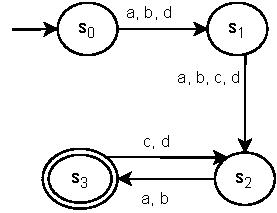
\includegraphics[height=100pt]{mintermization_automaton_m1.pdf}
        \caption{Finite automaton $A_1$ with transitions $\delta_1$.}
        \label{fig:diagram:mintermization_automaton_m1}
    \end{minipage}
    \hfill
    \begin{minipage}{0.47\linewidth}
        \centering
        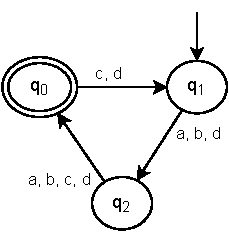
\includegraphics[height=100pt]{mintermization_automaton_m2.pdf}
        \caption{Finite automaton $A_2$ with transitions $\delta_2$.}
        \label{fig:diagram:mintermization_automaton_m2}
    \end{minipage}
    \vspace{0.5cm}
    \caption{Finite automata $A_1$ and $A_2$ used as example automata for mintermization.}
    \label{fig:diagram:mintermization_automata}
\end{figure*}

\begin{figure*}[ht]
    \centering
    \begin{minipage}{0.47\linewidth}
        \centering
        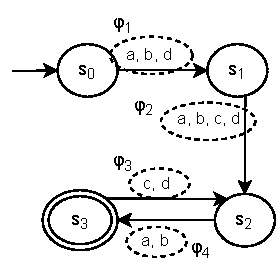
\includegraphics[height=100pt]{mintermization_automaton_m1_with_transition_sets.pdf}
        \caption{Finite automaton $A_1$ with transition sets $\varphi_i$.}
        \label{fig:diagram:mintermization_automaton_m1_with_transition_sets}
    \end{minipage}
    \hfill
    \begin{minipage}{0.47\linewidth}
        \centering
        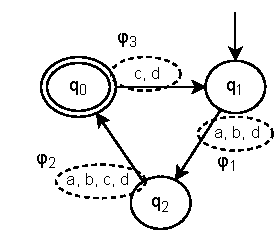
\includegraphics[height=100pt]{mintermization_automaton_m2_with_transition_sets.pdf}
        \caption{Finite automaton $A_2$ with transition sets $\varphi_i$.}
        \label{fig:diagram:mintermization_automaton_m2_with_transition_sets}
    \end{minipage}
    \vspace{0.5cm}
    \caption{Finite automata $A_1$ and $A_2$ with marked transition sets used in mintermization.}
    \label{fig:diagram:mintermization_automata_transition_sets}
\end{figure*}

Computation of minterms for $A_1$ and $A_2$ is illustrated in Figure~\ref{fig:diagram:mintermization_example} in a diagram.

\begin{figure}[ht]
	\centering
	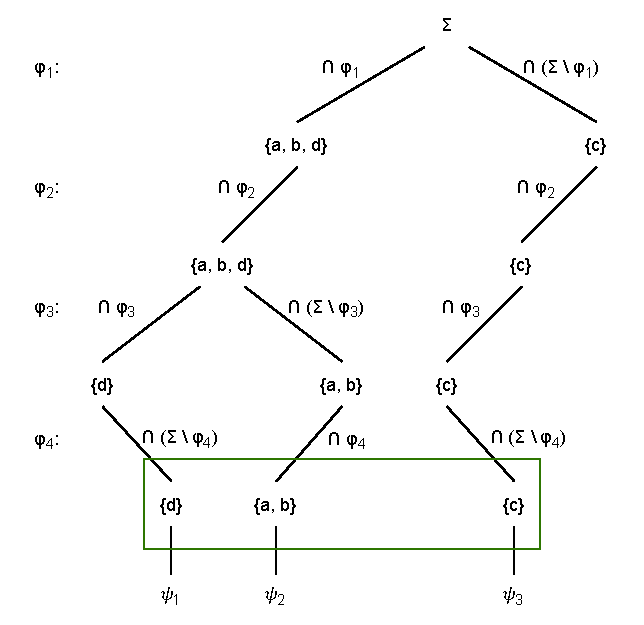
\includegraphics[]{mintermization_example.pdf}
	\caption{Mintermization process executed on example finite automata $A_1$ and $A_2$. We start with the whole alphabet and make our way down through all mintermization sets $\varphi_i$, where $1 \leq i \leq n$. For each mintermization set, we compute the intersection of the preceding set with the current mintermization set $\varphi_i$. The results are shown in the diagram as the nodes of the tree. When operations on all mintermization sets were executed, the leaves of the tree (indicated by the green square) represent the final minterms for the given mintermization sets $\Phi$ over the given alphabet $\Sigma$. We denote each minterm $\psi_i$, where $1 \leq i \leq |\Psi|$ where $|\Psi|$ represents the total number of generated minterms.}
	\label{fig:diagram:mintermization_example}
\end{figure}

We start with the whole alphabet of both automata\footnote{If the automata had non-equal alphabets, we would start with their intersection: $\Sigma = \Sigma_1 \cap \Sigma_2$. This is an optimization specific to product construction: If some transition symbols are not used by every finite automaton, we can safely omit such symbols as they are definitely not present in the intersection of these automata.} at the top of the minterm tree to be generated. Afterwards, we iterate over transition sets. For each transition set $\varphi_i$, we compute the intersection of the current minterm tree leaves with:
\begin{itemize}
    \item the current transition set $\varphi_i$ and store the result as a left node of this particular tree node,
    \item the complement of the current transition set $Q \setminus \varphi_i$ and store the result as a right tree node of this particular tree node.
\end{itemize}

If the intersection is empty, we omit creating the corresponding child node entirely. In the end, we are left with a complete minterm tree for the given set of transition sets $\Phi$ representing the specified finite automata.

The acquired minterms are:
$$ \Psi = Minterms(\Phi) = \bigl\{ \{d\}, \{a, b\}, \{c\} \bigr\} = \{ \psi_1, \psi_2, \psi_3 \} \text{.}$$

We can now substitute the former transition sets $\varphi_i$ for finite automata with the appropriate minterms $\psi_j, 1 \leq j \leq |\Psi|$ which were created from the specific transition sets $\varphi_i \in \Phi$ such that $\varphi_i$ is used in its direct form (not as a complement) in the process of computing $\psi_j$ (optimized for product construction). The gained automata can be seen in Figure~\ref{fig:diagram:mintermization_automata_with_minterms}.

\begin{figure*}[ht]
    \centering
    \begin{minipage}{0.47\linewidth}
        \centering
        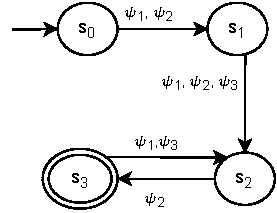
\includegraphics[height=100pt]{mintermization_automaton_m1_with_minterms.pdf}
        \caption{Finite automaton $A_1$ with transitions substituted by corresponding minterms $\psi_i \in \Psi$ created from these transition sets.}
        \label{fig:diagram:mintermization_automaton_m1_with_minterms}
    \end{minipage}
    \hfill
    \begin{minipage}{0.47\linewidth}
        \centering
        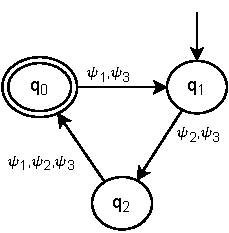
\includegraphics[height=100pt]{mintermization_automaton_m2_with_minterms.pdf}
        \caption{Finite automaton $A_2$ with transitions substituted by corresponding minterms $\psi_i \in \Psi$ created from these transition sets.}
        \label{fig:diagram:mintermization_automaton_m2_with_minterms}
    \end{minipage}
    \vspace{0.5cm}
    \caption{Finite automata $A_1$ and $A_2$ with substituted transitions with minterms in the process of mintermization.}
    \label{fig:diagram:mintermization_automata_with_minterms}
\end{figure*}

As we can see, we are able to get rid of some transition symbols and reduce the alphabet as well as the number of transitions in finite automata. Considering we have minterms over alphabet of $A$, we know that the intersection of two minterms has to be an empty set and that $\forall \psi \in \Psi ( \psi \subseteq \varphi, \varphi \in \Phi )$ if $\psi$ is created from $\varphi$. Important improvement of using minterms in product construction is the fact that $|\Psi| \leq |\Sigma|$ instead of at most $2^{|\Sigma|}$ as is the case for minterms over general predicates for general operation (e.g.,~\cite{minterms_forms-FITPUB11801}). We make use of these points further.

We can use the method of minterm computation with length or Parikh image abstractions of state languages. We choose this approach in order to improve pruning capabilities of length abstraction for some finite automata or speed up demanding Parikh image computation, especially for automata with multitude of transitions between two states varying only in transition symbols, which require considerate time to compute and evaluate.

This method proceeds to represent such sets of transitions between two states with (ideally) only a single minterm representing these transitions. We can therefore apply any previously mentioned optimization methods (or any other optimization method) on such modified automata with minterms as their transition symbols to construct their product without the need to compute, for example, Parikh image with every single transition symbol between two states. We can now compute possibly fewer transitions with the acquired minterms instead. Worst case is that the minterms do not reduce any transition symbols and we continue with the same, unchanged original automata. Minterm computation is quick and practically free optimization, which can be used every time an intersection of finite automata is computed.

We apply the minterm computation before we start executing any optimized algorithms introduced here or any others. Instead of putting original automata as the input to optimized algorithms, we compute minterms for such automata and substitute all transitions with the generated minterms. The new input to optimized algorithms are automata with minterms which can be easier to work with, and their intersection can be computed quickly and more precisely. If we need to use the intersection automaton further, not just to resolve the emptiness problem, we simply substitute the minterms in the product with the corresponding original transition symbols back.

Mintermization of our benchmark automata used in our experiments is however not useful, as the benchmark automata do not have multiple transitions between two states which could be changed into a minterm. Nevertheless, it is not hard to imagine instances of problems where minterms are essential.

For instance, take regular expressions. If we want to use our abstractions on finite automata representing regular expressions, we have to use mintermization in advance. Otherwise, gained abstractions would be extremely complex to evaluate for even simple regular expressions. Mintermization would allow us to modify such automata into finite automata with manageable number of transitions and transition symbols.

As a future work, we want to try our abstractions in optimizing automata operations in string solving methods such as~\cite{10.1007/978-3-319-08867-9_10} or~\cite{DBLP:conf/popl/LinB16}. These methods generate regular expressions with rich alphabets and complex transitions with character classes, which would be unsolvable for state language abstractions which have to consider each transition and its symbol.

As an example, imagine a simple regular expression $a[a-z]^*c.^*$ with its finite automaton. It contains numerous transitions for each of the symbols in character classes. Our abstractions would have to compute with each specific transition symbol. However, if we use mintermization on the automaton first, most of the transitions would be simplified into a few minterms: $\{ a \}$, $\{ c \}$, $\{ b, d-z \}$ and $\{ \beta \}$ where $\beta$ represents a set of the remaining symbols of $.^*$ not included in the previous minterms. Instead of complex automata transitions, we now have a finite automaton with only four transition symbols and eleven transitions. Our abstractions can now easily evaluate compatibility of such regular expressions.

%--------------------------------------------------------
%--------------------------------------------------------
%--------------------------------------------------------
%--------------------------------------------------------
\chapter{Experiments}\label{experimentsAndResultsChapter}

The reference implementation\footnote{In the \href{https://codeberg.org/Adda/optifa}{reference implementation}, we use \href{https://github.com/Z3Prover/z3}{Z3} as an SMT solver and automata operations are handled by for our purposes modified \href{https://codeberg.org/Adda/symboliclib}{library Symboliclib}.} of the proposed optimizations, written in Python 3, as well as a complete table of all of our experiments and their results and graphs is publicly accessible on a \href{https://codeberg.org/Adda/optifa}{Codeberg repository}\footnote{\url{https://codeberg.org/Adda/optifa}}.

Benchmark with sets of different finite automata used on our benchmark problems are available on a \href{https://github.com/ondrik/automata-benchmarks/tree/master/nfa/non-vtf/armc}{GitHub repository}\footnote{\url{https://github.com/ondrik/automata-benchmarks/tree/master/nfa/non-vtf/armc}}. These finite automata are obtained from runs of regular model checking tool on verification of pointer program and parametric protocols created in~\cite{model_checking_tool_10.1007/978-3-540-70844-5_7} based on method of abstract regular model checking from~\cite{method_model_checking_tool}. Such verification runs often execute operations similar to emptiness problem or product construction.

Our experiments cover the benchmark automata from 40 various categories of verification runs. In the benchmark, there are in total 5707 finite automata. However, each category contains similar finite automata recognizing similar languages. The results of our experiments on our benchmark problems for different combinations of finite automata from the same category are nearly identical. Thus, we choose representative finite automata from each category randomly. In total, we have executed more than 300 various experiment runs for combinations of more than 600 finite automata (over 300 pairs of two finite automata from one category). A timeout of 10 minutes for a single test was used.

We test combinations of finite automata from each category to determine the product construction and decide the emptiness of the finite automata intersection. In our experiments, our main objective is to find out how much our optimizations reduce product state space in both our benchmark problems. We want to know what are the pruning capabilities of both our optimizations and whether they are efficient. Further, we want to compare pruning capabilities of length abstraction and Parikh image abstraction to see whether Parikh image pruning capabilities are higher and by how much.

Our abstractions implemented by the reference implementation are not mature enough to properly compete in reduction of time cost of computation yet. Future work includes efficient implementation and further optimizations of our abstractions. Nevertheless, our experiments show our optimizations can sometimes speed up the execution of both benchmark problems.

In this chapter, we present a few experiments which show and compare the pruning capabilities of our optimizations on our benchmark problems. Second, we show what impact have optimizations on our abstractions on computation time on our both benchmark problems.

\section{Length Abstraction}

In our first experiment, we want to find out what are the pruning capabilities of length abstraction for both our benchmark problems on our benchmark automata. The graph in Figure~\ref{fig:graph:et_pruning_state_space_sizes_comp} shows a comparison of product state spaces sizes in unoptimized product construction and our optimized algorithm considering length abstraction for emptiness problem. The graph in Figure~\ref{fig:graph:fp_pruning_state_space_sizes_comp} shows a comparison of product state spaces sizes for unoptimized product and product optimized by length abstraction.

\begin{figure*}[ht]
    \centering
    \begin{minipage}{0.49\linewidth}
        \centering
        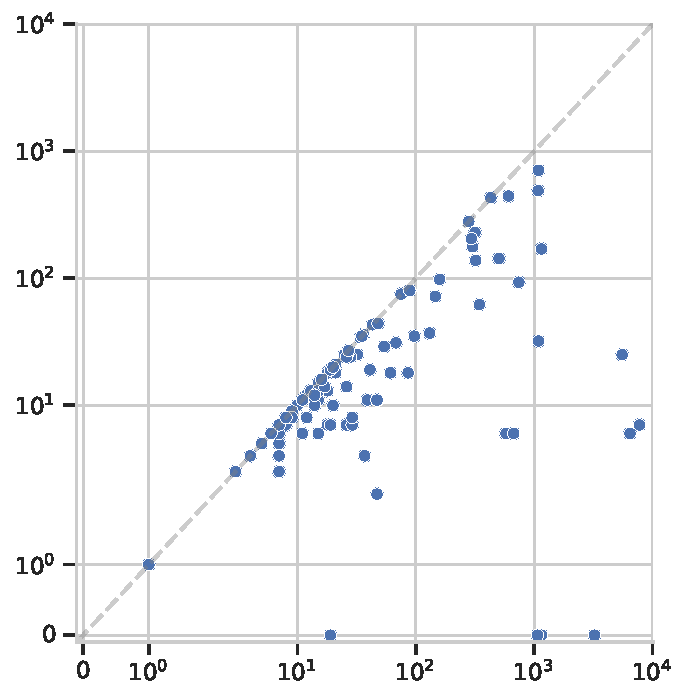
\includegraphics[scale=0.4]{graph_la_pruning_et_scatter.pdf}
        \caption{Emptiness problem.}
        \label{fig:graph:et_pruning_state_space_sizes_comp}
    \end{minipage}
    \hfill
    \begin{minipage}{0.49\linewidth}
        \centering
        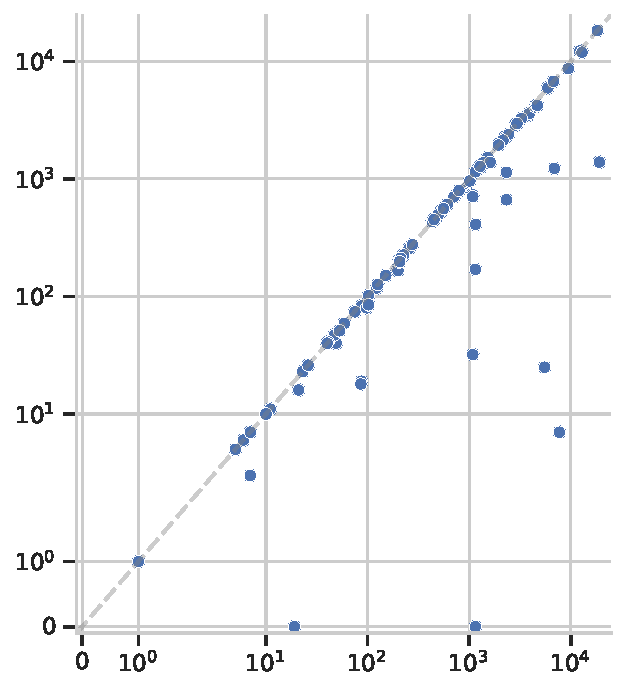
\includegraphics[scale=0.4]{graph_la_pruning_fp_scatter.pdf}
        \caption{Product construction.}
        \label{fig:graph:fp_pruning_state_space_sizes_comp}
    \end{minipage}
    \vspace{0.5cm}
    \caption{Comparison of state space sizes generated by unoptimized product and product optimized by length abstraction for both benchmark problems. Both axes are in symmetrical logarithmic scale\protect\footnotemark, x-axis showing the number of states generated by the unoptimized algorithms, y-axis state space sizes of the optimized algorithms.}
    \label{fig:graph:product_state_space_sizes}
\end{figure*}
\footnotetext{Plot is linear around $0$ instead of logarithmic.}

As we can see, length abstraction successfully prunes state space in some cases. The improvement can be seen especially for the emptiness problem. Notice that for some cases, length abstraction can stop product generation immediately on the first product state. However, if finite automata have large density of final states, they often accept plenty of different word lengths and length abstraction can have problems with finding incompatible abstractions.

The results where length abstraction have difficulties with pruning product space are influenced by our benchmark automata. The combinations of benchmark automata in each category rarely have empty intersections. Therefore, for our next experiment, we want to see whether slight modifications of input automata can highlight the strengths of length abstraction. To further extend the set of benchmark automata for this experiment, to each category, we add finite automata with slight modifications which we combine with original representatives in our experiments. These modifications imitate generation of variations of the same finite automata with different final states (similar to finite automata generated by string solving method from~\cite{10.1007/978-3-319-08867-9_10}) or little modifications of transitions (removed transitions or changed transition symbols). We want to observe whether length abstraction can notice the difference in finite automata and react accordingly by pruning the generated state space.

The following graphs show the results of intersection of combinations of the modified benchmark automaton with the original representative from each category for both deciding the emptiness problem and product construction. The graph in Figure~\ref{fig:graph:et_state_space_sizes_comp} shows the comparison of product state spaces sizes in unoptimized and our optimized product construction for emptiness problem. The graph in Figure~\ref{fig:graph:fp_state_space_sizes_comp} shows the comparison of product state spaces sizes in unoptimized and our optimized product construction for product construction.

\begin{figure*}[ht]
    \centering
    \begin{minipage}{0.49\linewidth}
        \centering
        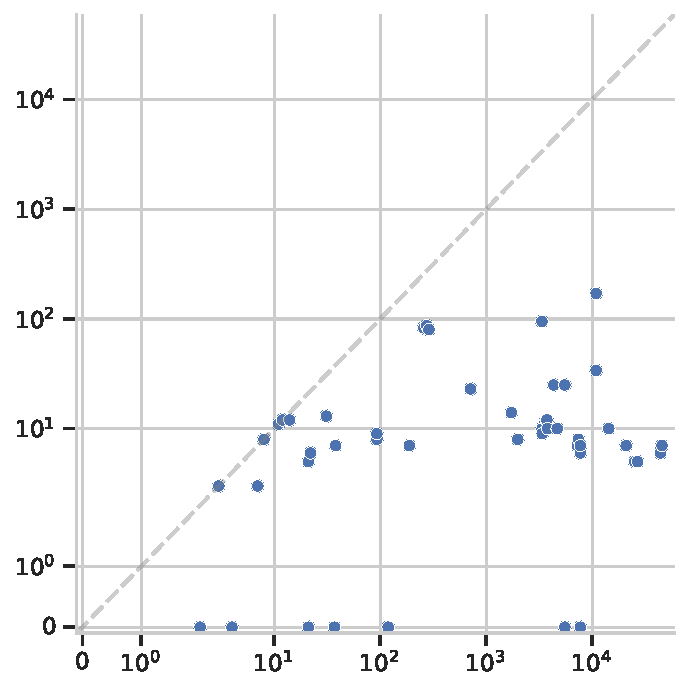
\includegraphics[scale=0.4]{graph_la_pruning_et_scatter_modifications.pdf}
        \caption{Emptiness problem.}
        \label{fig:graph:et_state_space_sizes_comp}
    \end{minipage}
    \hfill
    \begin{minipage}{0.49\linewidth}
        \centering
        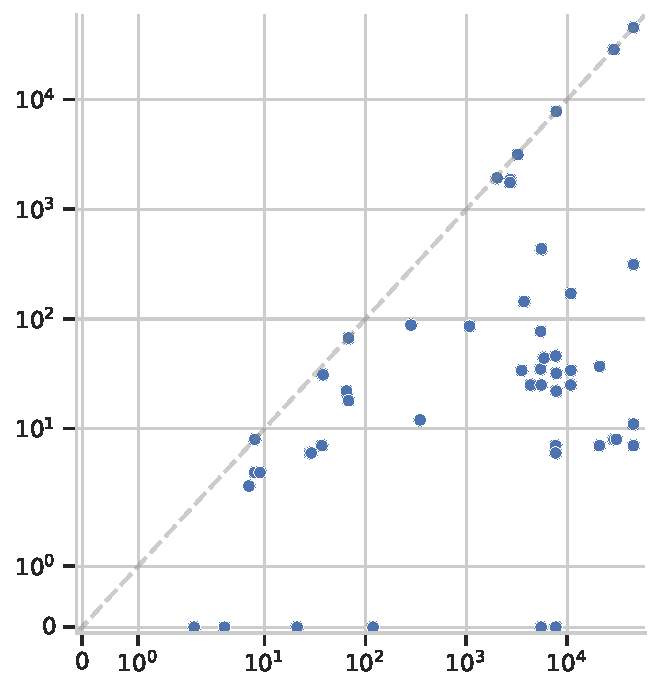
\includegraphics[scale=0.4]{graph_la_pruning_fp_scatter_modifications.pdf}
        \caption{Product construction.}
        \label{fig:graph:fp_state_space_sizes_comp}
    \end{minipage}
    \vspace{0.5cm}
    \caption{Comparison of state space sizes generated by unoptimized product and product optimized by length abstraction of both our benchmark problems with modification of benchmark automata. Both axes are in symmetrical logarithmic scale, x-axis showing the state space size of the unoptimized product, y-axis state space size of the optimized product.}
    \label{fig:graph:product_state_space_sizes}
\end{figure*}

Length abstraction is able to prune state space here more often, and the pruning capabilities of length abstraction are sufficient for these automata. We conclude that length abstraction can usually notice the difference between modified and original automata and truly prunes substantial parts of the newly unnecessary state space, which we might have created by our modifications. We can see from the graphs that the larger the unoptimized product gets, the higher impact length abstraction has on the product state space size. Product construction optimized by length abstraction generates much smaller products. Length abstraction accomplishes to eliminate state space explosion in most cases.

It is worth mentioning that we have neglected the number of generated states for our lasso automata. Their states are not in the product, but they are required for computation of the product. As we can see in Figure~\ref{fig:graph:product_state_space_sizes_with_lasso}, even when counting with lasso states, the total number of generated states in the whole process of the product construction can be lower than the unoptimized product state space size. The larger the automata are, the better results we get. It is understandable that for smaller original automata, the overhead of generating lasso automata is significant in comparison with the small generated product state space sizes. However, the larger the original automata get, the lesser the overhead of the number of lasso states is in comparison with the unoptimized product state space.

\begin{figure*}[ht]
    \centering
    \begin{minipage}{0.49\linewidth}
        \centering
        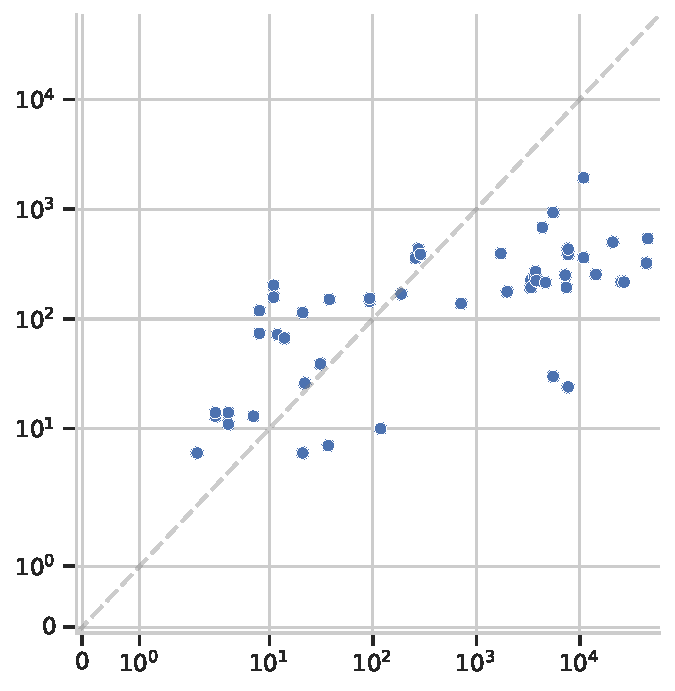
\includegraphics[scale=0.4]{graph_la_pruning_et_scatter_modifications_lasso.pdf}
        \caption{Emptiness problem.}
        \label{fig:graph:et_state_space_sizes_comp_with_lasso}
    \end{minipage}
    \hfill
    \begin{minipage}{0.49\linewidth}
        \centering
        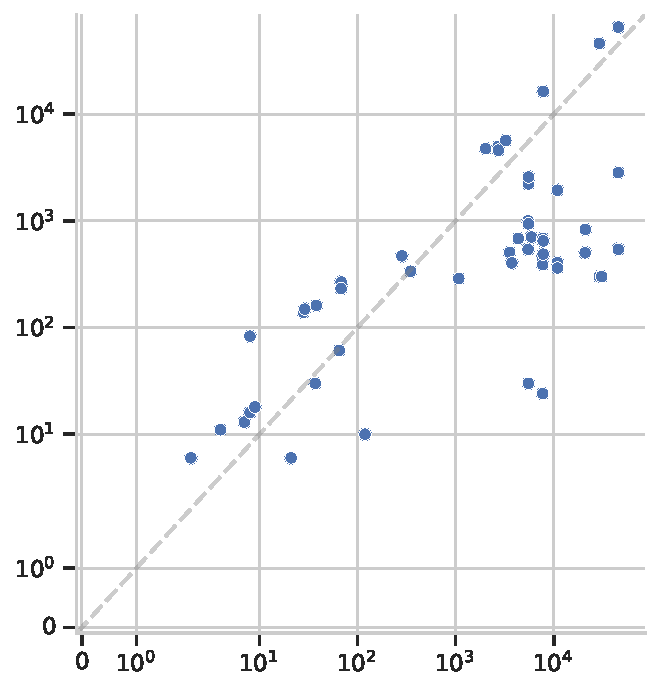
\includegraphics[scale=0.4]{graph_la_pruning_fp_scatter_modifications_lasso.pdf}
        \caption{Product construction.}
        \label{fig:graph:fp_state_space_sizes_comp_with_lasso}
    \end{minipage}
    \vspace{0.5cm}
    \caption{Comparison of state space sizes in unoptimized product and product optimized by length abstraction with a sum of states generated for both lasso automata. Both axes are in symmetrical logarithmic scale, x-axis showing the number of states in the unoptimized product, y-axis the number of states in the optimized product.}
    \label{fig:graph:product_state_space_sizes_with_lasso}
\end{figure*}

We can see that even that the overhead of generating lasso automata for length abstraction is necessary, if length abstraction can prune product states, it still pays off: The number of total states generated for either the product or lasso automata is smaller than the number of states in the unoptimized product.

For the rest of our experiments, we use only the original unmodified automata again.

\subsection{Length Abstraction Optimization without SMT solver}

We optimize evaluation of compatibility of length abstractions by substituting SMT solver with solving linear congruence equations. To show how linear congruences speed up the evaluation of compatibility of length abstractions on the original benchmark automata, we present the following experiment.

The Figure~\ref{fig:diagram:la_smt_difference} shows computation time from our benchmark problems pruned by length abstraction with and without SMT solver.

\begin{figure*}[ht]
	\centering
	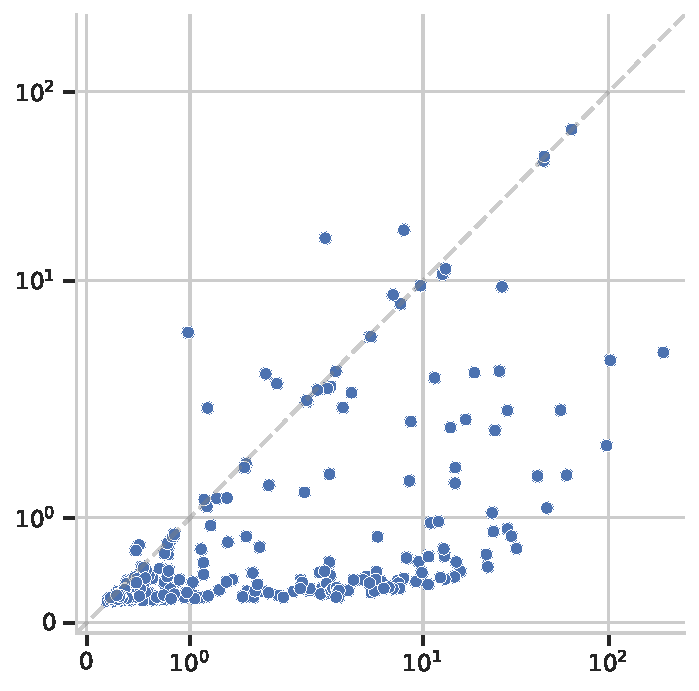
\includegraphics[scale=0.4]{graph_la_smt_difference.pdf}
	\caption{Comparison of time consumption of length abstraction evaluated by SMT solver and length abstraction evaluated without SMT solver, combining both benchmark problems. Both axes are in symmetrical logarithmic scale. They show time consumption in seconds: x-axis length abstraction evaluated by SMT solver, y-axis length abstraction evaluated without SMT solver.}
	\label{fig:diagram:la_smt_difference}
\end{figure*}

We can see that computation of both benchmark problems is faster for length abstractions solved by linear congruences. This optimization improves significantly computation time. Thus, whenever we use length abstraction, we should only evaluate compatibility with linear congruences instead of SMT solver.

Even though we do not focus on time cost of computation in our experiments, to get a first impression of how our optimized length abstraction compares to unoptimized product construction, we present an experiment in Figure~\ref{fig:diagram:basic_la_difference_time} showing the difference in time cost for unoptimized product construction and our optimized length abstraction.

\begin{figure*}[ht]
	\centering
	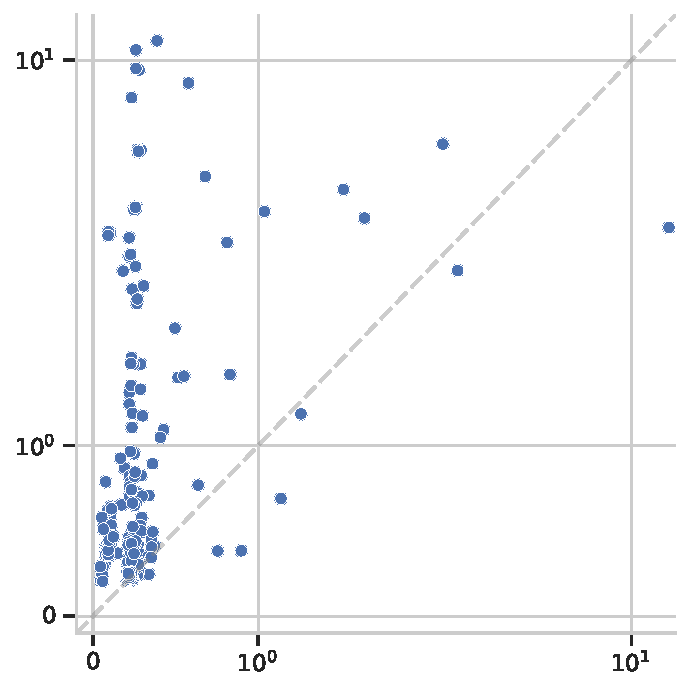
\includegraphics[scale=0.4]{graph_basic_la_time_difference.pdf}
	\caption{Comparison of time consumption of unoptimized product construction and length abstraction evaluated without SMT solver, combining both benchmark problems. Both axes are in symmetrical logarithmic scale. They show time cost in seconds: x-axis unoptimized product construction, y-axis length abstraction evaluated without SMT solver.}
	\label{fig:diagram:basic_la_difference_time}
\end{figure*}

As we can see, with length abstraction optimization of removing SMT solver, we can compute both our benchmark problems in time comparable to basic product construction. If parts of product construction can be pruned, we can even speed up both our benchmark problems. Our future work  includes further optimizing length abstraction to lower time cost to time comparable to unoptimized product construction or better for most cases, even when length abstraction cannot prune large state space.

Out of all experiments with length abstraction, one weakness of length abstraction is clear. The more final states the original automata have, the more difficult it is to optimize product construction using length abstraction. Every final state increases the number of accepted different lengths of automaton. Therefore, with automata where nearly every state is a final state, length abstraction cannot easily determine which product states can be pruned.

\section{Parikh Image Computation}

Length abstraction can sometimes prune product state space significantly, sometimes cannot. We introduced finer abstraction of state languages using Parikh images. Parikh image abstraction computes more precise over-approximation of the state language which would allow us to prune state space more often, even in cases where length abstraction fails. We aim at improving pruning capabilities of our abstractions. In this section, we show experiments with Parikh image abstractions. First, we are interested in pruning capabilities of Parikh image abstraction. Later, we evaluate optimizations of Parikh image abstraction.

We want to find out what are the pruning capabilities of Parikh image abstraction in both our benchmark problems on our benchmark automata. In Figure~\ref{fig:graph:pi_product_state_space_sizes_pruning_cap}, we can see how Parikh image prunes state space.
\begin{figure}[ht]
    \centering
    \begin{minipage}{0.49\linewidth}
        \centering
        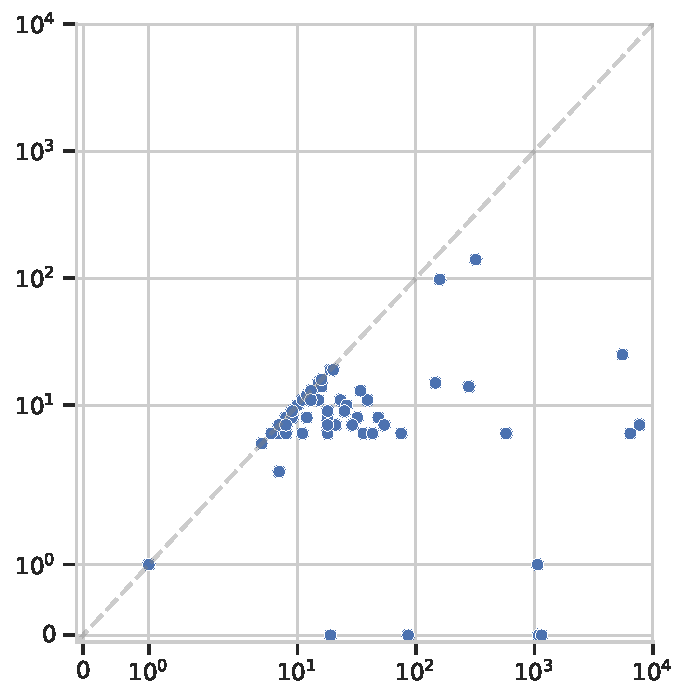
\includegraphics[height=150pt]{graph_pi_pruning_et_scatter.pdf}
        \caption{Emptiness problem.}
        \label{fig:graph:pi_et_state_space_sizes_comp}
    \end{minipage}
    \hfill
    \begin{minipage}{0.49\linewidth}
        \centering
        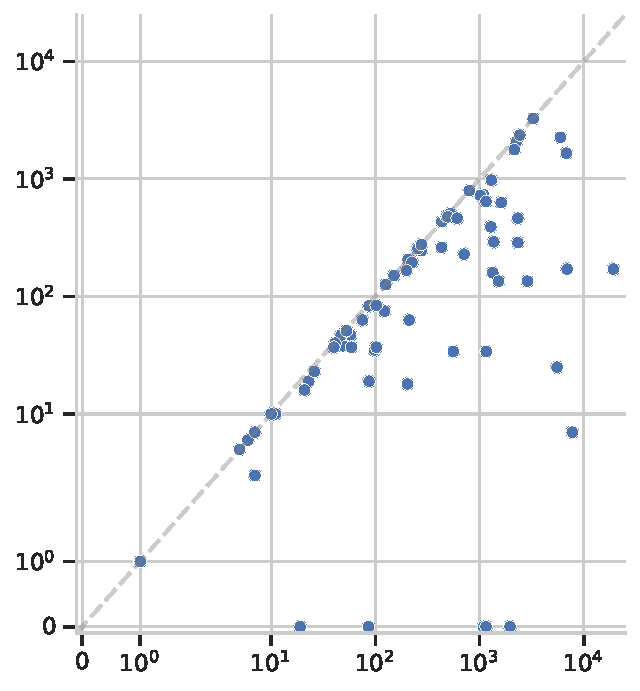
\includegraphics[height=150pt]{graph_pi_pruning_fp_scatter.pdf}
        \caption{Product construction.}
        \label{fig:graph:pi_fp_state_space_sizes_comp}
    \end{minipage}
    \vspace{0.5cm}
    \caption{Comparison of state space sizes generated by unoptimized product construction and product optimized with Parikh image abstraction. Both axes are in symmetrical logarithmic scale, showing state space sizes: x-axis of unoptimized product, y-axis of optimized product.}
    \label{fig:graph:pi_product_state_space_sizes_pruning_cap}
\end{figure}

We can see that Parikh image prunes the state space significantly in many cases and substantially more than length abstraction, especially for product construction problem. Notice that in some cases, Parikh image is able to stop product construction immediately for the initial product state. However, in total, Parikh image timed out 6 times on emptiness problem and 40 times on product construction. From this we can deduce, that Parikh image is able to decide emptiness problem even for complex automata. but, for product construction, Parikh image computation often takes significantly longer.

To see more clearly what is the difference in pruning capabilities of length and Parikh image abstractions, in the next experiment, we compare pruning capabilities of both abstractions between each other. The Figure~\ref{fig:diagram:pi_product_state_space_sizes} compares pruning capabilities of length and Parikh image abstractions.

\begin{figure}[ht]
	\centering
	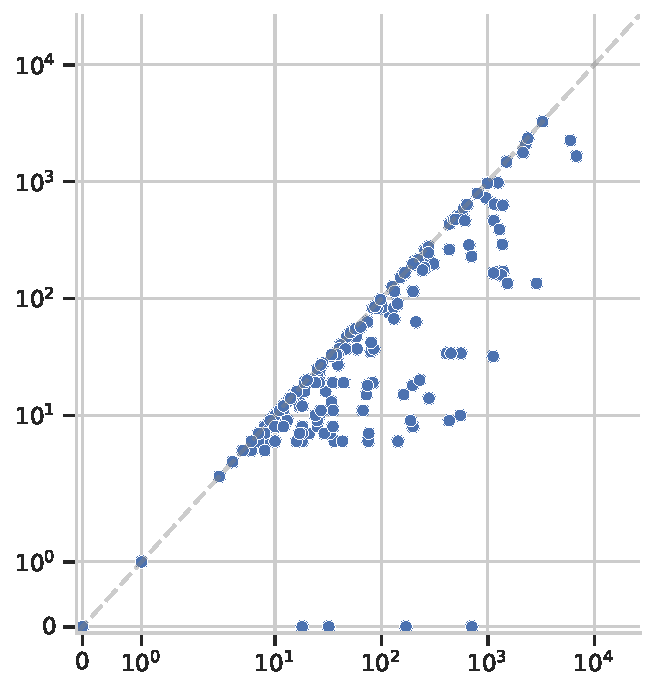
\includegraphics[scale=0.4]{graph_pi_la_comparison.pdf}
	\caption{Comparison of state spaces generated by length abstraction and Parikh image abstraction, combining both benchmark problems. Both axes are in symmetrical logarithmic scale. Axis show product state space sizes: x-axis for length abstraction, y-axis for Parikh image abstraction.}
	\label{fig:diagram:pi_product_state_space_sizes}
\end{figure}

Clearly, we can conclude from the experiment that Parikh image often optimizes the product state space more than length abstraction (at worst products are equal). Thus, pruning capabilities of Parikh image abstraction are higher than of length abstraction. In many cases, Parikh image optimization is able to prune vast state space by determining incompatible abstractions even if length abstractions are compatible. It is concluded that Parikh image is more precise abstraction, allowing us to prune more aggressively.

Furthermore, notice the dots at the bottom of the graph. Here, Parikh image is able to determine that product language is empty on the first product state and immediately stop the product construction even though length abstraction failed.

\subsection{Incremental SMT solving}

Incremental SMT solving proves to be a great improvement to the Parikh image computation optimization. We want to know how large part of Parikh image formulae can be precomputed and how many conjuncts have to be recomputed for each state. The number of conjuncts in Parikh images depends on the number of states in finite automata, the number of transitions and the number of initial or final states. See Table~\ref{table:incremental_smt_clauses} for an example comparison of the number of all conjuncts in Parikh image, conjuncts common to all states (persistent clauses) and state specific conjuncts (state specific clauses).

\begin{table*}[ht]
	\centering
	\small
    \begin{tabular}{ |c|c|c|c|c| }
        \hline
        Product States & All Conjuncts & Persistent Conjuncts & State Specific Conjuncts & Ratio \\ \hline
        434 & 2652 & 1782 & 870 & 67.2\% \\ \hline
    \end{tabular}
    \caption{An example proportion of persistent and state specific conjuncts in Parikh image computation with incremental SMT solving optimization. \emph{Product States} column shows the number of product states in the whole intersection product, \emph{All Conjuncts} column shows the number of conjuncts in each computed Parikh image, \emph{Persistent Conjuncts} column shows the number of persistent conjuncts in the whole Parikh image (out of the all Parikh image conjuncts), \emph{State Specific Conjuncts} column states how many Parikh image conjuncts have to be recomputed for each product state and \emph{Ratio} column shows the ratio of persistent conjuncts in all Parikh image conjuncts.}
    \label{table:incremental_smt_clauses}
\end{table*}

In this example, for a product of $434$ states, each product state Parikh image contains $2652$ conjuncts. From those, $1782$ conjuncts are persistent conjuncts and the remaining $870$ are state specific conjuncts. A proportional ratio of persistent conjuncts in whole Parikh image is around $67.2 \%$. The number of persistent conjuncts means around $70\%$ of computed Parikh image conjuncts can be precomputed once and used for the whole product generation, and SMT solver can use its cache for efficient evaluation of parts of the Parikh image formulae. Only $30\%$ of conjuncts must be computed repeatedly for each product state.

Even if our abstractions are not mature enough to properly optimize time cost, we want to get a first impression of what is the cost of more precise pruning capabilities of Parikh image abstraction in both our benchmark problems on our benchmark automata. In Figure~\ref{fig:graph:la_pi_time_cost_comp}, we can see how Parikh image optimized by incremental solving cost compares to length abstraction optimized by SMT solver substitution with solving linear congruences.
\begin{figure}[ht]
    \centering
    \begin{minipage}{0.49\linewidth}
        \centering
        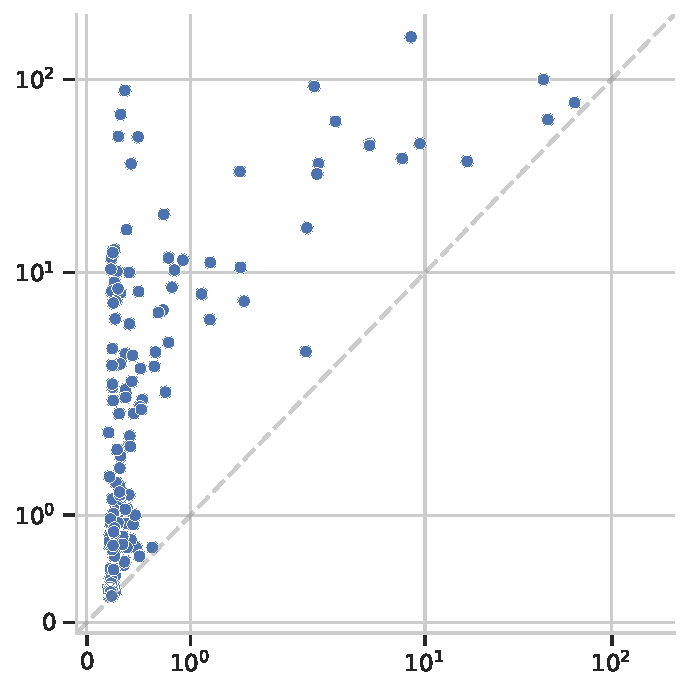
\includegraphics[height=150pt]{graph_la_pi_et_scatter_mean.pdf}
        \caption{emptiness problem.}
        \label{fig:graph:et_pi_la_comp_time_difference}
    \end{minipage}
    \hfill
    \begin{minipage}{0.49\linewidth}
        \centering
        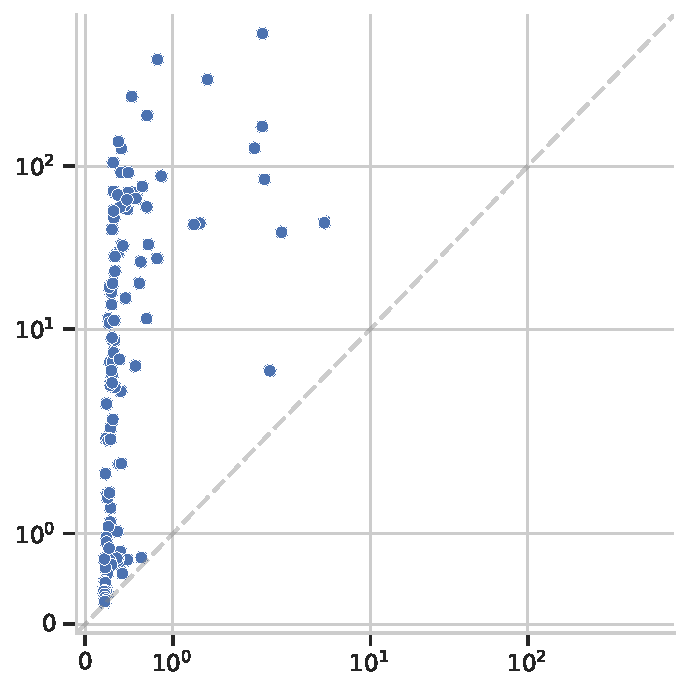
\includegraphics[height=150pt]{graph_la_pi_fp_scatter_mean.pdf}
        \caption{product construction.}
        \label{fig:graph:fp_pi_la_comp_time_difference}
    \end{minipage}
    \vspace{0.5cm}
    \caption{Comparison of the time cost of more precise pruning capabilities of Parikh image abstraction with incremental SMT solving and length abstraction optimized by SMT solver substitution with solving linear congruences. Both axes are in symmetrical logarithmic scale, showing time cost in seconds: x-axis of length abstraction, y-axis of Parikh image abstraction.}
    \label{fig:graph:la_pi_time_cost_comp}
\end{figure}

As we can see, the time cost for both problems is higher for Parikh image than for length abstraction. However, time cost of emptiness problem is less affected by the complexity of finite automata. For product construction, Parikh image may take longer to decide compatibility of all product states. We can conclude from the experiment that Parikh image time cost of more precise pruning capabilities is present, but in many cases, Parikh image is able to finish the solving of the problem in reasonable time.

\subsection{Precise Timeout Selection}

For our benchmark automata, we have experimentally concluded the ideal timeout for SMT solver to solve Parikh image abstractions compatibility is around $600$ ms. This gives SMT solver enough time to compute most incompatible cases, while it does not wait too long for the confirmation of satisfiability of Parikh image formulae for compatible cases. Our benchmark automata have however large numbers of transitions from each state, and therefore our timeout might not work best for other types of automata and their complexity. We suggest trying running our optimizations first without any timeout and then, according to the results, adjust the timeout according to the needs of given operations and the complexity of used automata.

\section{Combination of State Language Abstractions}

When we combine length and Parikh image abstraction optimizations in one algorithm, we want to help length abstraction to more precisely prune state space and reduce the number of product states for which Parikh image must be computed. In Figure~\ref{fig:diagram:combined_sat_unsat_comparison}, we can see how many product states can be skipped with our skippable states optimization, how many states is pruned by length abstraction and how many states is pruned by Parikh image abstraction (if length abstraction resolves length abstraction formulae as satisfiable). We provide comparison of pruning capabilities of both abstractions on the same automata.

\begin{figure}[ht]
	\centering
	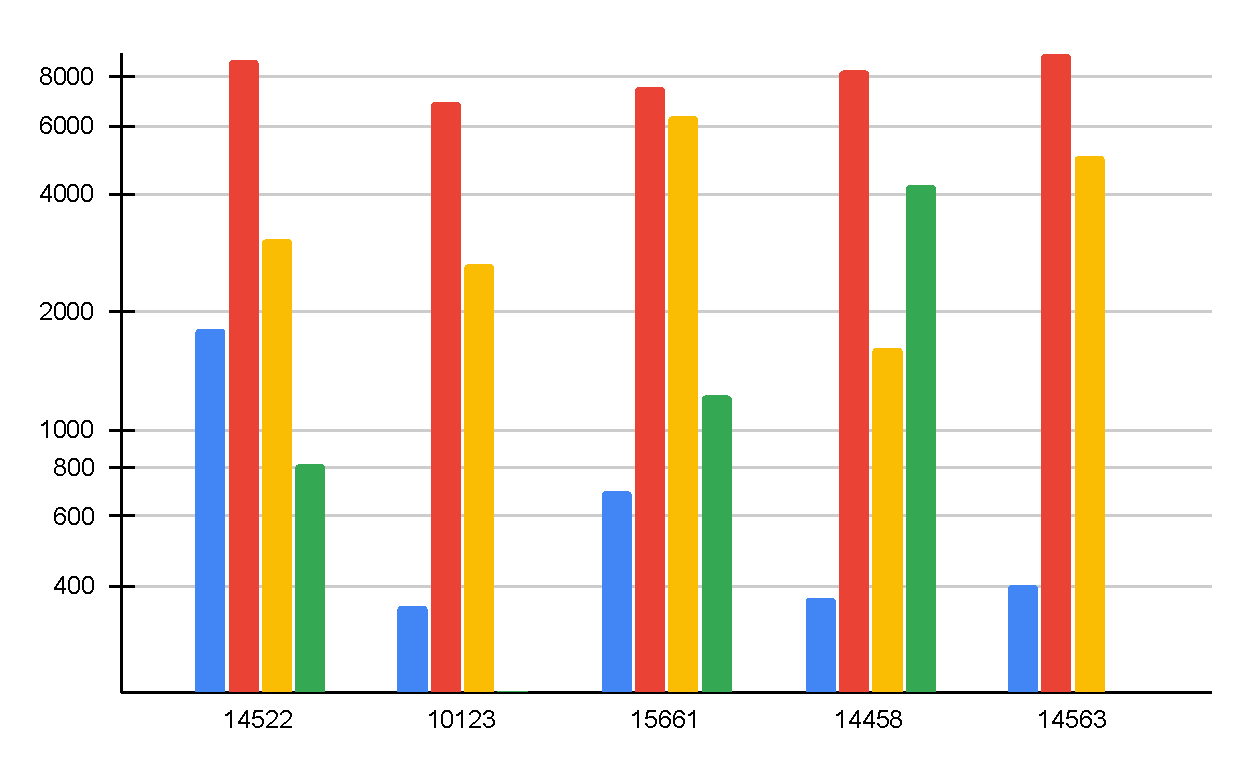
\includegraphics[scale=0.4]{combination_comparison_sats.pdf}
	\caption{Summary comparison of pruning capabilities of length and Parikh image state language abstractions in optimization algorithm combining both abstractions with optimizations by skippable states. Both axes are in the logarithmic scale: x-axis shows the number of processed product states in product construction (how many product states we have considered in total), y-axis the number of states resolved by respective abstractions. The blue column shows the number of skipped states (we do not need to evaluate abstractions for them), the red column the number of states with compatible both length and Parikh image abstractions, the yellow column the number of states pruned by Parikh image abstraction, but not by length abstraction, and the green column the number of states pruned by length abstraction alone. In the graph, we have summed the number of states resolved by each abstraction or optimization according to the number of processed states as follows (from left to right): $0$ to $499$, $500$ to $999$, $1000$ to $1999$, $2000$ to $2999$ and $3000+$.}
	\label{fig:diagram:combined_sat_unsat_comparison}
\end{figure}

We can clearly see that substantial number of states can be resolved by skippable states optimization or pruned by length abstraction. Parikh images do not have to be computed for any of these states. For the rest of the states, Parikh image have to be computed. We see here again how Parikh image abstraction is precise and helps when length abstraction cannot: Parikh image can prune large numbers of states even though length abstraction fails to prune them. The red and blue column together represent the number of states in the intersection, the yellow and green column the number of pruned states.

Notice that for the fourth column, for number of processed states between $2000$ and $2999$, length abstraction managed to prune extensive parts of product state space and therefore the number of product states pruned by Parikh image is clearly lower than for other categories. This shows that if length abstraction can prune the state space, there are less product states for Parikh image to resolve and therefore much less product states to be pruned by Parikh images. Length abstraction helped here substantially.

To sum it up, large parts of product can be pruned. We conclude that combined algorithm using both length abstraction Parikh image abstraction prunes state space really well.

To get an impression of how computation time is affected in product construction with Parikh image abstraction and with combined algorithm in both our benchmark problems on our benchmark automata, we present the following experiment. In Figure~\ref{fig:graph:pi_comb_time_cost_comp}, we can see how Parikh image cost compares to combined approach using both length and Parikh image abstractions.
\begin{figure}[ht]
    \centering
    \begin{minipage}{0.49\linewidth}
        \centering
        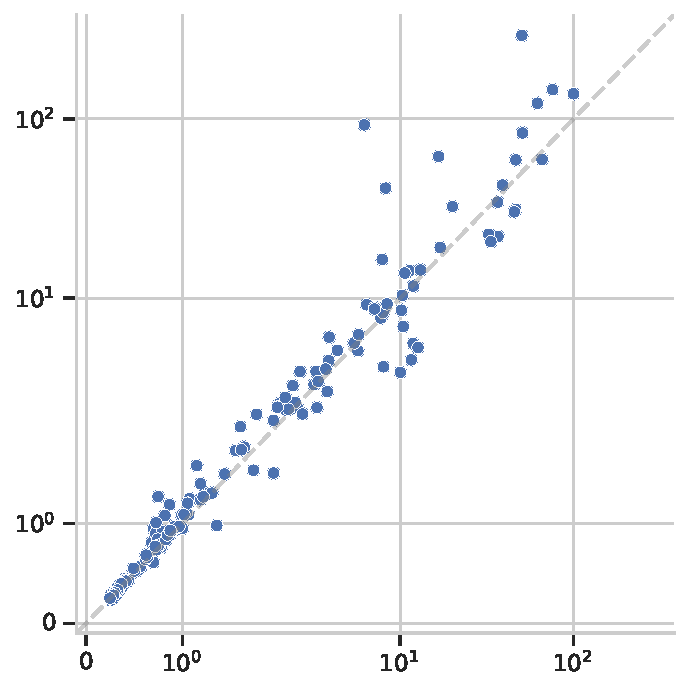
\includegraphics[height=150pt]{graph_pi_combined_et_scatter_mean.pdf}
        \caption{Emptiness problem.}
        \label{fig:graph:et_pi_comb_time_difference}
    \end{minipage}
    \hfill
    \begin{minipage}{0.49\linewidth}
        \centering
        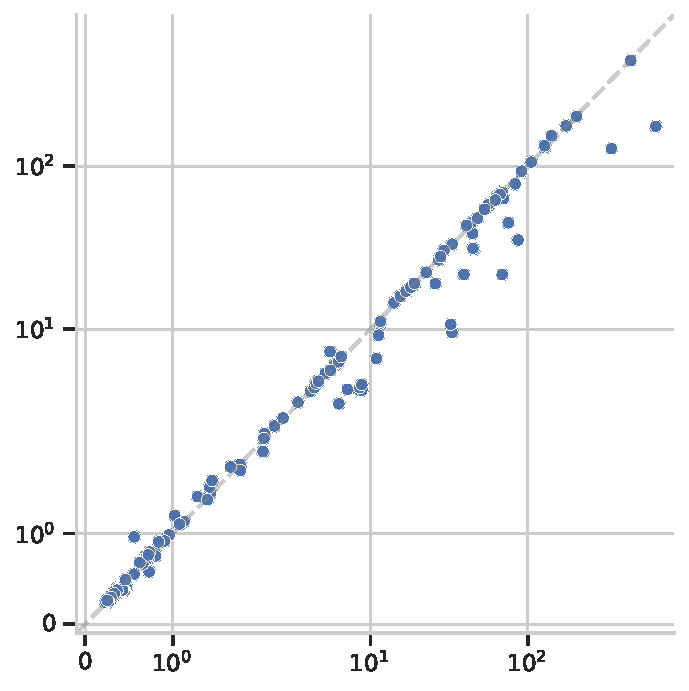
\includegraphics[height=150pt]{graph_pi_combined_fp_scatter_mean.pdf}
        \caption{Product construction.}
        \label{fig:graph:fp_pi_comb_time_difference}
    \end{minipage}
    \vspace{0.5cm}
    \caption{Comparison of the time cost of Parikh image abstraction and combined algorithm using both our abstractions. Both axes are in symmetrical logarithmic scale, showing time cost in seconds: x-axis of Parikh image abstraction, y-axis of combined algorithm.}
    \label{fig:graph:pi_comb_time_cost_comp}
\end{figure}

We can see that length abstraction pruning capabilities can help prune some product state which do not have to be evaluated by Parikh image abstraction and consequently speed up the product construction. There is also a cost of generating lasso automata with our abstractions, which can slightly increase the time cost in cases where there are no product state that can be pruned and both Parikh image and length abstraction have to be evaluated for each one of them.

We believe there is a space for further improvements to get better results with combined algorithm for every case. The key factor here is whether finite automata accept multitude of lengths. If they do, length abstraction cannot prune much and many evaluations of Parikh images have to be computed. On the other hand, if we had finite automata with empty intersections or accepting limited number of lengths, length abstraction can solve nearly the problem alone and Parikh image can be computed just for a few hard-to-resolve product states. This would significantly speed up the product construction.

\section{Results}


The experiments show that our abstractions often prune large parts of the product state space. Length abstraction pruning capabilities are decent, but sometimes it fails to prune state space for intersection of automata with multiple accepted lengths. Pruning capabilities of Parikh image are much higher. Parikh image often succeeds in pruning states where length abstraction fails. Further optimizations of the abstractions have impact on performance of our abstractions. State language abstractions are combinable without affecting pruning capabilities.

%--------------------------------------------------------
%--------------------------------------------------------
%--------------------------------------------------------
%--------------------------------------------------------
\chapter{Conclusion}

The most costly parts of the intersection computation is the generation of product states and transitions of the product automaton. We tried to reduce the size of the generated state space by pruning the states which cannot lead to any final state by deciding the emptiness of the corresponding state languages for the product states using various state language abstractions over the finite automata states, such as length abstraction using lasso automata or Parikh image computation based on Parikh's theorem. Our abstractions are based on over-approximating abstraction of state languages. Each approach has been experimentally tested and further optimizations to the proposed algorithms were introduced.

According to our experiments, product state space can be reduced substantially. Pruning capabilities of our abstractions are satisfactory, and their optimizations have high impact on computation time. We get great results especially for intersections with long lines or for intersections of automata which differ in accepted lengths. Experiments show our algorithm generates smaller state spaces for both resolution of emptiness problem and product construction.

We have concluded that length abstraction is fast and coarse abstraction, Parikh image precise but expensive. Our abstractions can be combined, parallelized and further extended.

Due to our discoveries, as a future work, we want to continue working on our state language abstractions, optimize their performance with efficient implementation and explore possibilities of additional improvements of these abstractions. We also want to parallelize evaluation of the compatibility of the abstractions. Further combinations with other abstraction techniques described below, to see how the generated product state space is affected, are in consideration, too.

The idea of using abstraction in automata problem-solving is not new, but it is not properly explored either. There were first attempts of using abstraction techniques in automata such as alternating automata~\cite{GANTY20103444} or abstract regular model checking~\cite{method_model_checking_tool, rmc_upside_down}, both using techniques similar to a general predicate abstraction~\cite{DBLP:conf/cav/ColonU98, DBLP:conf/cav/GrafS97} and CEGAR~\cite{DBLP:conf/cav/ClarkeGJLV00}.

However, we have not encountered similar approaches to optimization of product construction using length or Parikh image abstractions to compare our results with. Techniques using abstraction were explored especially in a field of program analysis. In the context of automata problem-solving are relevant namely CEGAR~\cite{DBLP:conf/cav/ClarkeGJLV00}, IC3/PDR~\cite{DBLP:conf/sat/HoderB12, DBLP:conf/fmcad/BradleyM07, DBLP:journals/pacmpl/HolikJLRV18, DBLP:conf/cav/WangTLYJ16, DBLP:journals/corr/abs-1708-09073} or IMPACT~\cite{DBLP:conf/cav/McMillan06}. There were some experiments using techniques similar to length abstraction using information about length constraints~\cite{10.1007/978-3-030-81688-9_14} to speed up string solving. There are also methods based on the interpolation-based approach of McMillan~\cite{DBLP:conf/tacas/AmlaM07, DBLP:conf/tacas/GangeNSSS13}. All the mentioned techniques have proven efficient in hardware or software verification, and they can be applied in automata too.

We believe state language abstractions introduced in this work are promising and their pruning capabilities have potential in various automata problems. For that reason, we will continue exploring this approach to automata problem-solving and investigate options of using state language abstractions to optimize operations on finite automata.
